% !TEX TS-program = xelatex
% !TeX spellcheck = en_GB
% !TeX root = ../My_thesis.tex

%\begin{algorithm}[!t]
%\caption{Pseudo-code for the first-order homogenisation scheme}
%\begin{mdframed}[style=algorithm]
%\begin{enumerate}[algorithm]  
%\item Calculate the effective stress and strain of the coarse scale
%\item Calculate the effective stress and strain of the coarse scale
%\item Calculate the effective stress and strain of the coarse scale
%\end{enumerate}
%\end{mdframed}
%\end{algorithm}


\chapter{Modelling Fibre-Reinforced Composites}\label{chap:math}

\section{Introduction}
	The performance of a material is measured through characterising its properties. The structure of the material, at every scale, affects these properties. Altering the structure happens under changing the manufacturing process, see Fig.~\ref{fig:tetra}. Correlating various structural entities to the material properties reveals the intricacies of the material response and enables the material engineer to adjust the performance under the stimuli. Obtaining experimental results is limited to the precision of equipment and feasibility of tests. Therefore, computational models could assist in obtaining the response of the material for a wide range of parameters. This alternative may provide a cost effective, yet insightful procedure, for material characterisation.
	
	Herein, the necessary preliminaries to material constitutive modelling used in the following chapters are concisely reviewed from the author's perspective. Then, the most common micromechanical modelling tools are briefly discussed within the scope of classical continuum mechanics (Cauchy media). Finally, the common bounding methods are revisited and the required formulations are derived. It is worth mentioning that where necessary, referrals are made to the relevant literature that is included in the following chapters. Therefore, in the following sections, the necessary preliminaries are included to achieve a better understanding.

\begin{figure}
\centering
\begin{tikzpicture}[line join = round, line cap = round, line width=1pt]
\pgfmathsetmacro{\factor}{1/sqrt(2)};
\coordinate [label={[label distance=0.2cm]right:{Properties}}] (A) at (2,-1,-2*\factor);
\coordinate [label={[label distance=0.2cm]left:{Processing}}] (B) at (-2,-0.5,-2*\factor);
\coordinate [label={[label distance=0.2cm]90:{Structure}}] (C) at (0,2.5,2*\factor);
\coordinate [label={[label distance=0.2cm]-90:{Performance}}] (D) at (0,-1.,2*\factor);


\node [draw, shape = circle, fill=red] (O) at (0,0.2,0) {};


\draw[-, fill=blue!30, opacity=.5] (B)--(C)--(A)--cycle;
\draw[-, fill=red!30, opacity=.5, dashed] (A)--(D)--(B)--cycle;
\draw[-, fill=green!50, opacity=.5, dashed] (A) --(D)--(C)--cycle;
\draw[-, fill=orange!50, opacity=.5] (B)--(D)--(C)--cycle;

\draw []  (B)--(D)--(C)--cycle;
\draw[] (A)--(D)--(C)--cycle;

\foreach \i in {A,B,C,D}
\node [draw, shape = circle, fill=blue!75!white!50!red] at (\i) {};



\node [] (T) at ($(+3,+.8)+(O.north east)$) {{\textit{Characterisation}}};
\draw [-Latex, line width=0.25mm,anchor=east] ($(T.south west)+(0cm,0.2cm)$) -- (O.north east) ;



\foreach \i/\x/\prop in {E/0.2/Mechanical,F/0.5/Electrical,G/0.8/Thermal,H/1.1/Magnetic,I/1.4/Optical,J/1.7/Deteriorative}
  \node [align=left, anchor=west] (\i) at ($(A)+(2.5cm,1-\x)$) {\small\prop};
\draw [fbrac] (J.west) -- (E.west);

\foreach \i/\x/\prop in {K/0.2/Sub-atomic,F/0.5/Atomic structure,F1/0.8/Atomic arrangement (short- and long-range order),F2/1.1/Nanostructure,G/1.4/Microscopic,H/1.7/Macroscopic}
  \node [align=left, anchor=west] (\i) at ($(C.west)+(1.25cm,1.4-\x)$) {\small\prop};
\draw [fbrac] (H.west) -- (K.west);


%  \shadedraw [ball color = red!50!blue, thin] (A) circle (0.15);

\end{tikzpicture}
\caption{Material science/engineering paradigm represented as a tetrahedron.}\label{fig:tetra}
\end{figure}

\section{Mathematical Tools}

\subsection{Tensors}
    \paragraph{Invariance} A coordinate system represents an observer---provided that the time lapse between the events is irrelevant. By introducing a coordinate system, the means to assign coordinates to entities is provided. Coordinates represent an object in a coordinate system. Setting up different coordinate systems provides the observer with different presentations of the same object. Since all the representations refer to the same physical object, they are equivalent in a sense---or in a better term the object is \textit{invariant}~\autocite{Jaunzemis.1967}. 

    \paragraph{Transformation laws} Tensors are used to describe physical quantities. The tensorial representation is a combination of the basis of the coordinate system and some tensor components. Thus, changing the coordinate system will change both the coordinate bases and the components of a tensor. Demanding invariance from a tensor is done by enforcing equality between its two representations of the same quantity. The result is the \textit{transformation laws} by which invariant constructs are formed. More generally, invariance is achieved because of the inverse relationship between the Jacobians in transforming covariant and contravariant tensor components~\autocite{Grinfeld.2013}.

    \paragraph{Intuitive definition} Although the notion of invariance may be considered as the basic incentive for using tensors, other tensor properties intervene in defining tensors. In the literature, some tried to provide a definition by explaining the behaviour of a tensor under basis transformations whereas others focused more on its mapping functionality. Intuitively, a tensor is a mathematical object that encapsulates the following information:
    \begin{enumerate}
        \item the instructions for a linear mapping,
        \item associated components in terms of specific basis vectors, and
        \item the quality of being invariant under basis transformation.
    \end{enumerate}
    The components of a tensor are determined upon the selection of basis vectors and they change according to specific transformation rules from one set of basis to another. Therefore, components of a tensor are associated with its bases, i.e., they have unique components in a specific set of basis. These components will change if the basis vectors change. Nevertheless, components of a tensor together with its bases are invariant.
    
    \begin{definition}[Tensor]\label{def:tensors}
        A tensor $\ten{T}$ of  $n$-th order in the $d$-dimensional space is defined as a scalar-valued linear function of $n$ vectors:
        \begin{equation}
        \begin{aligned}
        \ten{T}: &\underbrace{\tena{u}\in\Real^d\times\tena{v}\in\Real^d\times\ldots  \times\tena{w}\in\Real^d}_n   \mapsto \alpha\in\Real\\
                  &\ten{T}[\tena{u},\tena{v},\ldots,\tena{w}]=\alpha,
        \end{aligned}
        \end{equation}
        where $d$ is the dimension of the space, and $\alpha$ is a scalar, and $n$ is the order (or rank) of the tensor which is denoted by $\order{\ten{T}}=n$. The dimension and the order of a tensor are expressed together as $\class{n}{d}$ which indicates the \textit{class} of a tensor, i.e., the set of all $n$-th order $d$-dimensional tensors. Note that a more general class (set) is constructed by only indicating the order of a tensor such as $\class{n}{}$.\\
        Note that targeting a specific component of a tensor is denoted by several ways:
        \begin{equation}
        	T_{ij\ldots k}\equiv[\ten{T}]_{ij\ldots k}\equiv (\ten{T})_{ij\ldots k}.
        \end{equation}
    \end{definition}
    To emphasise on the linearity of tensors, one may add the following line to complement the definition:
    \begin{equation}
       \forall a,b,\ldots ,z\in \Real:\qquad\ten{T}[a\tena{u},b\tena{v},\ldots,z\tena{w}]=ab\ldots z\,\ten{T}[\tena{u},\tena{v},\ldots,\tena{w}].
    \end{equation}

	\paragraph{Link to conventions} Based on the definition of class of a tensor, some infamous sets in classical continuum mechanics~\autocite{Bertram.2012} can be re-expressed as
    \begin{subequations}
    \begin{alignat}{3}
%        \linset         &=\,&                     &\class{2}{3},\\
%        \linpset        &=\,& \null^+             &\class{2}{3},\\
%        \symset         &=\,& \null^\text{s}      &\class{2}{3},\\
%        \orthset        &=\,& \null^\text{o}      &\class{2}{3},\\
%        \sympset        &=\,& \null^{\text{s}+}   &\class{2}{3},\\
%        \orthpset       &=\,& \null^{\text{o}+}   &\class{2}{3},\\
%        \skwset         &=\,& \linset &- \symset,
         \linsettext         &=\,&& \linset,         \\
         \linpsettext        &=\,&& \linpset,        \\
         \symsettext         &=\,&& \symset,         \\
         \orthsettext        &=\,&& \orthset,        \\
         \sympsettext        &=\,&& \sympset,        \\
         \orthpsettext       &=\,&& \orthpset,       \\
         \skwsettext         &=\,&& \skwset,\\
         \unisettext         &=\,&& \uniset,
    \end{alignat}
    \end{subequations}
    where `$+$' is denotes the set of all tensors with a positive determinant, `sym' indicates the symmetrical tensors, and `orth' indicates the orthogonal tensors. The anti-symmeteric (skew-symmetric) set is defined as $\skwset \equidef \linset - \symset$. The unimodular set $\uniset$ indicates all second-order tensors with a determinant value of $\pm1$.





% ══════════════════════════════════════════════════════════════════════════════════════════════════
\subsection{Operations}
    \paragraph{Inner product} In linear algebra, the inner product is a real-valued bilinear map of two vectors for which the dot product is the standard choice. Namely, the inner product---as a primary concept and a norm---is used to set up the space. Thereby, the secondary concepts of length and angle are defined. The resulting space is an Euclidean space which is nothing but a real space equipped with the concepts of inner product and norm. The former is denoted by $\Euclid$ whereas the latter is denoted by $\Real$ to emphasise on this arrangement; however, they are often used interchangeably~\autocite{Tadmor.2012,Grinfeld.2013}.

    \begin{definition}[Inner Product]
        In tensor analysis, the inner product is a binary operation over two tensors which is often shown by the dot symbol ($\scp$). For instance, the tensor $\ten{T}$ is applied consecutively on several vectors to map them to a scalar:
        \begin{equation}\label{eq:contr}
            \ten{T}[\tena{v},\ldots,\tena{w}] \equiv \ten{T} \odot (\tena{v} \dyad  \ldots \dyad \tena{w})=\mathcal{T}_{i\ldots j}v_{i} \ldots w_j.
%            \ten{T}[\tena{v},\ldots,\tena{w}]\equiv \ten{T}(\tena{v},\ldots,\tena{w}) \equiv \ten{T} \odot (\tena{v} \dyad  \ldots \dyad \tena{w})=\mathcal{T}_{i\ldots j}v_i \ldots w_j.
        \end{equation}
        The power of a tensor is calculated by the inner product:
        \begin{equation}
        \ten{T}^n=\underbrace{\ten{T}\scp\ldots\scp\ten{T}}_{n-1\ \text{inner products}},\qquad\qquad\forall n\in\Integer^+.
        \end{equation}
%        or in the full component notation as
%        \begin{equation*}\label{eq:arb_trans}
%            \ten{T}  \scp\tena{v} \scp  \ldots \scp \tena{w} 
%                \equiv (\mathcal{T}_{i\ldots j}\base_i\dyad \ldots\dyad\base_j) \scp\null(v_k \base_k) \scp \ldots \scp\null (w_l \base_l) 
%                \equiv \mathcal{T}_{i\ldots j}v_i \ldots w_j.
%        \end{equation*}
    \end{definition} 
    Note that as a result of the inner product, the indexes of vector and tensor components are made equal---it is called \textit{contraction} of the indexes. The inner product is called the \textit{scalar product}, the \textit{dot product} and \textit{composition} too. Particularly, if all the free tensor indexes are contracted by consecutive dot products, the operation is called a scalar product to emphasize on the nature of the obtained entity. Similarly, the term `composition' is used because of its resemblance to that of the functions. Assume that linear vector fields
\begin{equation}
A(\tena{x}), B(\tena{x}),\ldots, Z(\tena{x}): \tena{x}\in\Real^d \mapsto \Real^d,
\end{equation}
have the tensorial equivalents $\tenb{A}, \tenb{B},\ldots,\tenb{Z}$. According to the representation theory~\autocite{Brannon.2017}, the function composition of
\begin{equation}
A\circ B\circ \ldots \circ Z(\tena{x}),
\end{equation}
will be equivalent to its tensorial form
\begin{equation}
\tenb{A}\scp \tenb{B}\scp \ldots \scp \tenb{Z}\scp \tena{x}.
\end{equation}
Although the resemblance exists in a sense, the composition of functions maps onto the same space whereas in the tensorial form this concept applies only to the second-order tensors. Moreover, sometimes `composition' refers to the outer product, e.g., $A_{ij}v_k$ and what is meant here as composition is called \textit{transvection}, i.e., a composition followed by a contraction such as $A_{ij}v_j$, c.f.~\autocite{Jaunzemis.1967,Haupt.2002}. The literature regarding the tensor calculus is not univocal---at least not in terms of notation.

\red
In the frame of reference $(o,\base_i)$, a tensor maps the basis vectors to is components, i.e., passing the basis vectors to a tensor reveals its components:
\begin{equation}
\ten{T}[\base_i,\ldots,\base_j]\equiv \ten{T}\scp\ldots\scp (\base_i \dyad \ldots \dyad \base_j) \equiv \mathcal{T}_{j\ldots i}.
\end{equation}
Tensors of class $\class{2}{3}$ occur frequently in continuum mechanics and are used to map a vector to another vector by a single contraction:
\begin{equation}
\tenb{A}[\tena{v}]\equiv \tenb{A}(\tena{v}) \equiv \tenb{A} \scp \tena{v} \equiv A_{ij}\base_i\dyad\base_j\scp v_k\base_k = A_{ij}v_j \base_i.
\end{equation}
In the partial component notation, the basis vectors are ignored and only the components are shown. Herein, straight brackets are used to denote the components of a symbol and discard the basis vector in the notation:
\begin{equation}
[\tenb{A} \scp \tena{v}]_i \equiv A_{ij}v_j,
\end{equation}
where obviously one subscript is added to the left-hand side for every basis being removed. Clearly, two consecutive contractions of the same second-order tensor result in a scalar:
\begin{equation}
\tenb{A}[\tena{v},\tena{u}]\equiv \tenb{A}(\tena{v},\tena{u}) \equiv \tenb{A} \scp \tena{v} \scp \tena{u}\equiv A_{ij}\base_i\dyad\base_j\scp v_k\base_k \scp u_l\base_l = A_{ij}v_ju_i.
\end{equation}
Note that in this case there is no need to to use the $[\op]_i$ style since there are no basis vectors, i.e., the result is a scalar since all the indexes are contracted.
\bl




\paragraph{Outer product} The outer product is used to create higher order entities. For instance, a dyad is built from the outer product of two vectors. A dyadic is a sum of dyads. Every dyadic is a tensor and every tensor can be represented by a dyadic but not uniquely. 

\begin{definition}[Outer product]
    Multiplying two variants results in another variant. Such a product is called an \textit{outer product} or a \textit{tensor product}:
    \begin{equation}
    \ten{A}=\ten{B}\dyad\ten{C}.
    \end{equation}
    As a result of tensorial product, the order of the result is increased, i.e., $\order{\ten{A}}
    =\order{\ten{B}}+\order{\ten{C}}$.
        The tensorial power of a tensor is calculated by the outer product:
        \begin{equation}
        \ten{T}^\tenpow{n}=\underbrace{\ten{T}\dyad\ldots\dyad\ten{T}}_{n-1\ \text{outer products}},\qquad\qquad\forall n\in\Integer^+.
        \end{equation}    
\end{definition}


\paragraph{Cross product} Replacing an outer product in a dyadic reduces the order of the tensor by one. However, the more important property of the cross product is in creating a vectorial invariant that is closely related to the notion of a pseudo-tensor.
\begin{definition}[Cross product]
The cross products maps two vectors ($\tena{u}$ and $\tena{v}$) into a third vector 
\begin{equation}
\tena{\omega}=\tena{u}\times\tena{v},
\end{equation}
where the result is perpendicular to the plane of the original vectors, and its direction is determined based on the handedness of the coordinate system. 
\end{definition}
\red
Replacing an outer product in a dyadic reduces the order of the tensor by one. However, the more important property of the cross product is in creating a vectorial invariant which is closely related to the notion of a pseudo-tensor.

	A skew-symmetric tensor $\tenb{A}^\skw\in\class{2}{d}$ has only a $d$-number of independent components, and thus it can be represented by the pseudo-vector $\tena{\omega}\in\class{1}{d}$---so called the \textit{vectorial invariant} associated with the tensor (or simply the associated vector). The vectorial invariant is obtained from
\begin{equation}
\tena{\omega}=-\frac{1}{2}\levi\dscp\tenb{A}^\skw,\label{eq:skw}
\end{equation}
or alternatively using Gibbs cross~\autocite{Lurie.1990}
\begin{equation}
\tena{\omega}=-\frac{1}{2}\gibbs{\tenb{A}}.
\end{equation}
Thus, it is evident that the axial vector of a second order skew-symmetric dyadic is the cross product of the corresponding dyads: 
\begin{equation}
-\frac{1}{2}\gibbs{(\tena{u}\dyad\tena{v}-\tena{v}\dyad\tena{u})}=\tena{v}\cross\tena{u},
\end{equation}
which can be used to replace a cross product by its skew-symmetric dyadic or on the other hand, the original tensor can be replaced by its vectorial invariant:
\begin{alignat}{2}
&\forall \tena{x}\in\class{1}{d}:&\qquad\tenb{A}^\skw\scp\tena{x}=\tena{\omega}\times \tena{x},
\end{alignat}
for the price of involving a pseudo-vector but of a lower order. Note that the symmetrical part of $\tenb{A}$ does not play a role in Gibbs cross since contracting a symmetrical and a skew-symmetrical tensor of the same class vanishes:
\begin{equation}
\tenb{A}^\sym\dscp\tenb{B}^\skw=0,
\end{equation}
and thus the axial invariant of a symmetric tensor is nil:
\begin{equation}
\gibbs{(\tenb{A}^\sym)}=\nulla.
\end{equation}
Finally, the alternative notations for Gibbs cross are \autocite{Assmus.2017b}
\begin{equation}
\gibbs{\tenb{A}}\equiv \tenb{A}\times\scp\,\unitb\equiv\levi\dscp\tenb{A}=\tenb{A}\dscp\levi, % \tenb{A}\boxtimes\unitb
\end{equation}
where $\levi$ is the Levi-Civita symbol defined as
\begin{equation}
\levi\equidef\epsilon_{ijk}\base_i\dyad\base_j\dyad\base_k=\base_i\cross\base_j\scp\base_k.%,\qquad\text{with}\quad 
\end{equation}
	Alternatively, the result of the cross product of a vector with the unit tensor is a skew-symmetric tensor:
	\begin{equation}
		\tenb{A}^\skw = \unitb\cross\tena{\omega},
	\end{equation}
	which can be derived from Eq.~\eqref{eq:skw}.\bl


% ══════════════════════════════════════════════════════════════════════════════════════════════════
\paragraph{Transposition} The transpose ($\op^\tran$) or conjugate (for complex tensors) is an operation which changes the dyadic order of a tensor. While transposing 1st-order tensors is irrelevant, only one type of transpose can be defined for a second-order tensor $\tenb{T}$: 
\begin{equation}
\forall \tena{u},\tena{v}\in \class{1}{n}:\qquad \tena{u}\scp\tenb{T}\scp\tena{v}=\tena{v}\scp\tenb{T}^\tran\scp\tena{u}.
\end{equation}
The common operation of transposing can be extended to fourth-order tensors $\tend{C}$ where it is called the main transpose:
\begin{equation}
\forall \tenb{A},\tenb{B}\in \class{2}{n}:\qquad \tenb{A}\scp\tend{C}\scp\tenb{B}=\tenb{B}\scp\tend{C}^\tran\scp\tenb{A}.
\end{equation}
Other high-order transpose operations are
\begin{subequations}\label{eq:transpose}
\begin{alignat}{2}
[\tend{C}^\tran ]_{ijkl}\equidef C_{klij}&\qquad\text{(main) transpose},    \\
[\tend{C}^\ttran]_{ijkl}\equidef C_{lkji}&\qquad\text{total transpose},    \\
[\tend{C}^\ltran]_{ijkl}\equidef C_{jikl}&\qquad\text{left transpose}, \\
[\tend{C}^\rtran]_{ijkl}\equidef C_{ijlk}&\qquad\text{right transpose},\\
[\tend{C}^\mtran]_{ijkl}\equidef C_{ikjl}&\qquad\text{middle transpose},\\
[\tend{C}^\otran]_{ijkl}\equidef C_{ljki}&\qquad\text{outer transpose}.
\end{alignat}
\end{subequations}
\paragraph{Symmetry} The symmetry of a tensor is nothing but its invariance under a transpose operation. The most common form is that under the main transposition:
\begin{subequations}
\begin{alignat}{2}
\tenb{T}=\tenb{T}^\tran&\qquad \text{or}\quad&   T_{ij}&=T_{ji},    \label{eq:tran2}\\
\tenc{T}=\tenc{T}^\tran&\qquad \text{or}\quad&   T_{ijk}&=T_{kji},  \label{eq:tran3}  \\
\tend{C}=\tend{C}^\tran&\qquad \text{or}\quad& C_{ijkl}&=C_{klij},\label{eq:tran4}
\end{alignat}
\end{subequations}
where $\tenb{T}$ is symmetrical and $\tend{C}$ has main (major) symmetry. The total symmetry along with sub-symmetries (minor symmetries) can be achieved by enforcing the following equalities:
\begin{subequations}
\begin{alignat}{2}
\tend{C}^\tran \equimust\tend{C} &\qquad\text{(main or major) symmetry},    \\
\tend{C}^\ttran\equimust\tend{C} &\qquad\text{total symmetry},    \\
\tend{C}^\ltran\equimust\tend{C} &\qquad\text{left subsymmetry}, \\
\tend{C}^\rtran\equimust\tend{C} &\qquad\text{right subsymmetry},\\
\tend{C}^\mtran\equimust\tend{C} &\qquad\text{middle subsymmetry},\\
\tend{C}^\otran\equimust\tend{C} &\qquad\text{outer subsymmetry}.
\end{alignat}
\end{subequations}


\paragraph{Conjugation product} This type of product is a variation of the outer product and is encountered during index permutation for symmetrisation/anti-symmetrisation~\autocite{Akivis.1977} of tensors.

\begin{definition}[Conjugation product]
    The conjugation product is dual to the tensor product. Two forms are available in literature: 
    \begin{enumerate}
    \item A dyadic product followed by a middle transpose\footnote{Often the symbol $\conj$ is used, see~\autocite{Guidugli.2000} for instance.}
        \begin{equation}
            (\tenb{A}\dyadu\tenb{B})\equidef(\tenb{A}\dyad\tenb{B})^\mtran.
        \end{equation}
        This product is also called the `tensor product of transformations'~\autocite{Halmos.1974}, i.e., its application to the outer product of the two vectors (a second-order tensor) is equivalent to separately transforming each of these vectors by means of the second order tensors:
        \begin{equation}
        \tenb{A}\dyadu\tenb{B}\dscp(\tena{u}\dyad\tenb{v})= (\tenb{A}\scp\tena{u})
        \dyad(\tenb{B}\scp\tenb{v}),
        \end{equation}
        or
        \begin{equation}
        (\tenb{A}\dyadu\tenb{B})\dscp\tenb{T}= \tenb{A}\scp\tenb{T}\scp\tenb{B}^\tran.
        \end{equation}        
    \item A dyadic product followed by a right transpose and a middle transpose
        \begin{equation}
            (\tenb{A}\dyado\tenb{B})\equidef\big((\tenb{A}\dyad\tenb{B})^\rtran\big)^\mtran,
        \end{equation}
        which applies the the following transformation
        \begin{equation}% TODO double check
%        (\tenb{A}\dyado\tenb{B})\dscp\tenb{T}= \tenb{A}\scp\tenb{T}^\tran\scp\tenb{B}^\tran.
        (\tenb{A}\dyado\tenb{B})\dscp\tenb{T}= \tenb{A}\scp\tenb{T}\scp\tenb{B}.
        \end{equation}              
    \end{enumerate}
	Finally, a symmetric dyadic product is defined as
        \begin{equation}
        \tenb{A}\dyadd\tenb{B}\equidef \frac{1}{2}(\tenb{A}\dyadu\tenb{B}+\tenb{A}\dyado\tenb{B}).
        \end{equation}              	
%   The following lines are not correct 100%:    
%    or equivalently
%    \begin{equation}
%        (\tenb{A}\dyadu\tenb{B})\scp\tenb{C}\equidef\tenb{A}\scp\tenb{C}\scp\tenb{B}^\tran.
%    \end{equation}
\end{definition}



% ══════════════════════════════════════════════════════════════════════════════════════════════════
%\subsection{Defining the Transpose Operation}
%	For a second-order tensor:
%	\begin{alignat}{2}
%		\forall \tena{x}, \tena{y}\in\class{1}{d}&\quad \wedge\quad& \forall \tenb{A}\in\class{2}{d}:&\qquad \tena{x}\scp\tenb{A}\scp\tena{y}\equimust \tena{y}\scp\tenb{A}^\tran\scp\tena{x},
%	\end{alignat}
%	or equivalently:
%	\begin{alignat}{2}
%		x_iA_{ij}x_j=y_jA_{ji}^\tran x_i\quad\rightarrow\quad A_{ij}=A_{ji}^\tran.\tag{\ref{eq:tran2} revisited}
%	\end{alignat}
%	The notion can be extended to third-order tensors:
%	\begin{alignat}{2}
%		\forall \tena{x}, \tena{y}\in\class{1}{d}& \quad \wedge\quad& \forall \tenc{A}\in\class{3}{d}:&\qquad \tena{x}\scp\tenc{A}\scp\tena{y}\equimust \tena{y}\scp\tenc{A}^\tran\scp\tena{x},
%	\end{alignat}
%	and consequently:
%	\begin{alignat}{2}
%		x_iA_{ijk}y_k=y_kA_{kji}^\tran x_i \quad\rightarrow\quad A_{ijk}=A_{kji}^\tran.\tag{\ref{eq:tran3} revisited}
%	\end{alignat}	
%	For fourth-order tensors, double-dot product (either horizontal or vertical) is used to extract the notion of transposing. For a vertical double-dot product:
%	\begin{alignat}{2}
%		\forall \tenb{A}, \tenb{B}\in\class{2}{d}& \quad \wedge\quad& \forall \tend{T}\in\class{4}{d}:&\qquad \tenb{A}\dscp\tend{T}\dscp\tenb{B}\equimust \tenb{B}\dscp\tend{T}^\tran\dscp\tenb{A},
%	\end{alignat}	
%	or equivalently:
%	\begin{alignat}{2}
%		A_{ij}T_{ijkl}B_{kl}=B_{kl}T_{klij}^\tran A_{ij}
%		\quad\rightarrow\quad T_{ijkl}=T_{klij}^\tran.\tag{\ref{eq:tran4} revisited}
%	\end{alignat}	
%	For a horizontal double-dot product:
%		\begin{alignat}{2}
%			\forall \tenb{A}, \tenb{B}\in\class{2}{d}& \quad \wedge\quad& \forall \tend{T}\in\class{4}{d}:&\qquad \tenb{A}\dhscp\tend{T}\dhscp\tenb{B}\equimust \tenb{B}\dhscp\tend{T}^\tran\dhscp\tenb{A},
%		\end{alignat}	
%		or equivalently:
%		\begin{alignat}{2}
%			A_{ji}T_{ijkl}B_{lk}=B_{lk}T_{klij}^\tran A_{ji}
%			\quad\rightarrow\quad T_{ijkl}=T_{klij}^\tran.\tag{\ref{eq:tran4} revisited}
%		\end{alignat}
%	Thus, using either type of double-dot product results in the same definition of the transposing operation.
%	
%	\paragraph{Positive-definiteness requirement of scalar products} According to the correspondences with Dr.~Sébastien Brisard, the horizontal double-dot product is not a scalar product since it does not produce a positive-definite form ($\tenb{A}\dhscp \tenb{A} \ge 0$). Only for zero tensors this equation form becomes zero. However, non-zero orthogonal tensors also produce a zero value when horizontal double-dot is used:
%	\begin{equation*}
%	\tenb{A}\dhscp \tenb{A} = \tenb{A}\dscp \tenb{A}^\tran = 0\quad \rightarrow\quad  \tenb{A}^\tran \equimust \tenb{A}^\inv.
%	\end{equation*}
%	A more descriptive proof should be acquired using Hilbert spaces.
% ══════════════════════════════════════════════════════════════════════════════════════════════════
\subsection{Projection Theorem}
Most profoundly useful engineering theorems are intuitively obvious but mathematically more complex. The \textit{projection theorem} says that a vector can be decomposed into another vector along a preferred direction (projection) plus what is left over (rejection). This is obvious in 3D vector space but it is also applicable to many other vector-like objects, e.g., tensors, matrices, and differentiable functions. In this regard, some applications of the projection theorem are~\autocite{Brannon.2003}:
\begin{itemize}
\item A scalar function can be written as the sum of odd and even parts, e.g., in Fourier series using two sets of orthogonal functions.
\item A matrix can be decomposed to symmetric and skew-symmetric components.
\item A continuously differentiable function can be expressed as a Taylor series.
\item Most material constitutive laws can be expressed in terms of projections in terms of volumetric and deviatoric components.
\end{itemize}
\begin{definition}[Projection Tensor]
The symmetric tensor $\tenb{P}$ is a projection tensor and the symmetric tensor $\tenb{P}^*$ is its complementary projection tensor if
\begin{subequations}
\begin{alignat}{4}
\forall n\in\Integer^+&:&                    \tenb{P}^n&=\tenb{P},&\quad&\text{idempotence,}\\
\forall n\in\Integer^+&:&           (\tenb{P}^*)^n&=\tenb{P}^\prime,&&\text{idempotence,}\\
                      & &      \tenb{P}+\tenb{P}^*&=\unitb,&&\text{completeness,}\\
                      & &  \tenb{P}\cdot\tenb{P}^\ast&=\nullb,&&\text{bi-orthogonality} .
\end{alignat}
\end{subequations}
These projections are of class $\class{2}{3}$ but the concept can be extended to higher order classes as well. 
\end{definition}
% ──────────────────────────────────────────────────────────────────────────────────────────────────
\paragraph{Unit tensors interpreted as projectors} The 1st-order unit vector (direction vector) is denoted by $\unita$\footnote{In 3D Euclidean coordinate systems, $\base_i$ denotes the basis vector for $i$-th axis which should not be confused with its components; for instance, $\base_1$ is the basis vector of 1-direction while its components are denoted by $[\base_1]_i$.} and has a unit length ($\norm{\unita}=1$). The 2nd-order unit tensor can be used as a trivial projection tensor:
\begin{equation}\label{eq:unitb}
\unitb\equidef\delta_{ij}\,\base_i\dyad \base_j,
\end{equation}
where $\delta_{ij}$ is Kronecker delta~\parencite{Itskov.2007}. Projection tensors of class $\class{4}{3}$ are 
\begin{subequations}
\begin{alignat}{5}
&\unitd      &\equidef&&\delta_{ik}\delta_{jl}                                    &&\,\base_i\dyad \base_j\dyad \base_k\dyad \base_l,\\
&\unitdT&\equidef&&\delta_{il}\delta_{jk}                                    &&\,\base_i\dyad \base_j\dyad \base_k\dyad \base_l,\\\label{eq:IRT}
&\unitd^\sym &\equidef&&\half(\delta_{ik}\delta_{jl}+\delta_{il}\delta_{jk})&&\,\base_i\dyad \base_j\dyad \base_k\dyad \base_l,\\
&\unitd^\skw &\equidef&&\half(\delta_{ik}\delta_{jl}-\delta_{il}\delta_{jk})&&\,\base_i\dyad \base_j\dyad \base_k\dyad \base_l,\\\label{eq:vol}
&\unitd^\vol &\equidef&&\third\delta_{ij}\delta_{kl}                         &&\,\base_i\dyad \base_j\dyad \base_k\dyad \base_l,\\
&\unitd^\dev &\equidef&&\half(\delta_{ik}\delta_{jl}+\delta_{il}\delta_{jk})-\third\delta_{ij}\delta_{kl}  &&\,\base_i\dyad \base_j\dyad \base_k\dyad \base_l.
\end{alignat}
\end{subequations}
	Alternatively, these 4th-order projectors can be represented in terms of their 2nd-order counterpart:
	\begin{subequations}
	\begin{alignat}{5}
	&\unitd			&=&\;&&\unitb\dyadu\unitb,\\
	&\unitdT		&=&&&\unitb\dyado\unitb,\\
	&\unitd^\sym	&=&&&\half(\unitb\dyadu\unitb+\unitb\dyado\unitb)=\unitb\dyadd\unitb=\half(\unitd+\unitdT),\\
	&\unitd^\skw	&=&&&\half(\unitb\dyadu\unitb-\unitb\dyado\unitb)=\half(\unitd-\unitdT),\\
	&\unitd^\vol	&=&&&\third \unitb\dyad\unitb,\\
	&\unitd^\dev	&=&&&\unitd^\sym-\unitd^\vol,
	\end{alignat}
	\end{subequations}
	where their relation is obtained using higher order transpose operations in Eq.~\eqref{eq:transpose}, e.g., $\unitdT= ((\unitd^\rtran)^\mtran)^\ltran$.
As projectors, the aforementioned tensors of $\class{4}{3}$ can operator on $\class{2}{3}$:
\begin{subequations}
\begin{alignat}{1}
	\unitd\dscp\tenb{T}	        	=&\tenb{T},\\
	\unitdT\dscp\tenb{T}   			=&\tenb{T}^\tran,\\
	\unitd^\vol\dscp\tenb{T}		=&\tenb{T}^\vol,\\
	\unitd^\dev\dscp\tenb{T}	 	=&\tenb{T}^\dev,
\end{alignat}
\end{subequations}
\red
\subsection{Gradient, Divergence, and Curl}
    The nabla (del) operator in 3D is defined as 
    \begin{equation}
        \tena{\nabla}\equiv\base_i\partial_{i}\equidef\base_i{\partial\over\partial x_i}.
    \end{equation}
    where $\partial_{i}$ is the partial derivative operator with respect to $i$-th coordinate; it enables a concise indicial notation such as~$\partial_{i}Q_{jk}=Q_{jk,i}$.
    
    Herein, the nabla operator is used to define the (left) gradient, divergence, and curl of the tensor field $\ten{T}\in\class{2}{3}$, respectively:
    \begin{subequations}
    \begin{alignat}{4}
        \diver{\ten{T}}                 
            &\equidef\; \base_m\partial_m\scp \ten{T}
            &=\;&\base_m\scp\,{\partial \mathcal{T}_{ij...k} \over x_m}\,\base_i\dyad\base_j\dyad\ldots\dyad\base_k,\\
        \symbf{\nabla}{\,\dyad\,\ten{T}}
            &\equidef\; \base_m\partial_m\dyad\ten{T}
            &=\;&\base_m\dyad {\partial \mathcal{T}_{ij...k} \over x_m}\,\base_i\dyad\base_j\dyad\ldots\dyad\base_k,\\
        \curl{\ten{T}}                  
            &\equidef\; \base_m\partial_m\cross\ten{T}
            &=\;&\base_m\cross{\partial \mathcal{T}_{ij...k} \over x_m}\,\base_i\dyad\base_j\dyad\ldots\dyad\base_k.
    \end{alignat}
    \end{subequations}
    In a similar fashion, the right gradient, divergence, and curl of the tensor field $\ten{T}$ can be defined:
    \begin{subequations}
    \begin{alignat}{4}
        \text{div}\,{\ten{T}}
            &\equidef\; \ten{T}\scp\symbf{\nabla}
            &=\;&\ten{T}\scp\base_m\partial_m
            &=\;&\mathcal{T}_{ij...k}\base_i\dyad\base_j\dyad\ldots\dyad\base_k\scp\base_m\,{\partial  \over x_m}\,\\
        \text{grad}\,{\ten{T}}      
            &\equidef\; \ten{T} \dyad\symbf{\nabla}
            &=\;&\ten{T}\dyad\base_m\partial_m
            &=\;&\mathcal{T}_{ij...k}\base_i\dyad\base_j\dyad\ldots\dyad\base_k\dyad\base_m\,{\partial  \over x_m}\,\\
        \text{curl}\,{\ten{T}}      
            &\equidef\; \ten{T} \cross\symbf{\nabla}
            &=\;&\ten{T}\cross\base_m\partial_m
            &=\;&\mathcal{T}_{ij...k}\base_i\dyad\base_j\dyad\ldots\dyad\base_k\cross\base_m\,{\partial  \over x_m}.
    \end{alignat}   
    \end{subequations}
    The aforementioned right and left quantities can be related. For instance, the right-gradient and left-gradient of a vector field $\tena{v}$ are related by
    \begin{equation}
        \text{grad}\,\tena{v}\equiv\tena{v}\dyad\symbf{\nabla}=(\symbf{\nabla}\dyad\tena{v})^\tran=(\grad{\tena{v}})^\tran.
    \end{equation}

\begin{comment}

     
The nabla (del) operator in 2D is defined as 
\begin{equation}
\tena{\nabla}_\text{S}\equiv\base_\alpha\partial_{\alpha}=\base_\alpha{\partial\over\partial x_\alpha},
\end{equation}
and similarly, all the mentioned definitions can be restated in their planar forms. For instance, applying the nabla operator on the same tensor field $\ten{T}\in\class{2}{3}$ but in the $X_1$-$X_2$ plane results in:
\begin{alignat}{4}
\sdiver{\ten{T}} &=\;&\base_\alpha&&\scp\,&&{\partial \mathcal{T}_{\beta\gamma...\lambda} \over x_\alpha}\,\base_\beta\dyad\base_\gamma\dyad\ldots\dyad\base_\lambda,\\
\sgrad{\,\ten{T}}  &=\;&\base_\alpha&&\dyad &&{\partial \mathcal{T}_{\beta\gamma...\lambda} \over x_\alpha}\,\base_\beta\dyad\base_\gamma\dyad\ldots\dyad\base_\lambda,\\
\scurl{\ten{T}}  &=\;&\base_\alpha&&\cross&&{\partial \mathcal{T}_{\beta\gamma...\lambda} \over x_\alpha}\,\base_\beta\dyad\base_\gamma\dyad\ldots\dyad\base_\lambda.
\end{alignat}
Finally, the surface operators can be related to their 3D counterparts. For example, the gradient of a scalar field $a$ can be related to its surface gradient on an arbitrary plane with the normal of $\tena{n}$:
\begin{equation}
\sgrad{a}=\grad{a}-\tena{n}(\tena{n}\scp\grad{a}).
\end{equation}
\end{comment}
\bl

%All the equations of this section can be transformed to class $\class{4}{2}$ by changing the letter `I' to `P' and using Greek subscripts. For instance, Eq.~\eqref{eq:unitb} is changed to 
%\begin{equation}
%\tenb{P}=\delta_{\alpha\beta}\,\base_\alpha\dyad \base_\beta,
%\end{equation}
%where $\tenb{P}$ is the unit tensor of the surface (first metric tensor) and it is used to project 3D tensors to 2D. As another example, Eq.~\eqref{eq:vol} can be written as
%\begin{equation}
%\tend{P}^\vol =\half\delta_{\alpha\beta}\delta_{\gamma\eta}   \,\base_\alpha\dyad \base_\beta\dyad \base_\gamma \dyad \base_\eta,
%\end{equation}
%or equivalently as
%\begin{equation}
%\tend{P}^\vol =\half\tenb{P}\dyad\tenb{P},
%\end{equation}
%where the coefficient $\sfrac{1}{3}$ is changed to $\sfrac{1}{2}$ to reflect the decrease in the dimension of the space.
%
%%───────────────────────────────────────────────────────────────────────────────────────────────────
%%\subsection{Interpreting Projection Tensors}
%Applying the projection tensor on tensors of class $\class{1}{3}$ and $\class{2}{3}$ will produce different results, and thus different interpretations are possible. For instance, the membrane stress components on the plane with the normal~$\tena{n}$ can be readily extracted by applying the first fundamental tensor of the surface ($\tenb{A}$) to the stress tensor ($\tenb{T}\in\class{2}{3}$):
%\begin{alignat}{2}
%&\tenb{A}\scp\tenb{T}\scp\tenb{A}&\hspace*{2cm}\text{with}\quad& \tenb{A}=\unitb-\tena{n}\dyad\tena{n}.
%\end{alignat}
%Similarly, the transverse shear components are extracted by
%\begin{equation}
%\tenb{A}\scp\tenb{T}-\tenb{A}\scp\tenb{T}\scp\tenb{A}.
%\end{equation}
%Note that the resulting shear tensor is not a symmetric one due to the presence of only two shear components.
%
%In contrast, a vector $\tena{v}$ can be projected along an arbitrary direction indicated by $\unita$ and the plane normal to this direction. As a result, the parallel component (projection vector) $\tena{v}^\parallel$ and the complementary perpendicular component (rejection vector) $v^\perp$ is obtained by
%\begin{alignat}{4}
%\tena{v}^\parallel &=& \tenb{P}^\parallel&\cdot \tena{v}     &&\qquad\text{with}\quad&        \tenb{P}^\parallel&=\unita\dyad\unita,\\
%\tena{v}^\perp    &=&     \tenb{P}^\perp&\cdot \tena{v}     &&\qquad\text{with}\quad&   \tenb{P}^\perp    &=\unitb-\unita\dyad\unita.
%\end{alignat}
%Note that $\tenb{P}^\perp$ and $\tenb{P}^\parallel$ are of class $\class{2}{3}$.
% &\text{4-th order unit tensor}          &\hspace*{0.5cm}&     
% &\text{transpose 4-th order unit tensor}&\hspace*{0.5cm}&     
% &\text{symmetric 4-th order unit tensor}&\hspace*{0.5cm}&     
% &\text{skew-symmetric 4-th order unit tensor}&\hspace*{0.5cm}&
% &\text{volumetric 4-th order unit tensor}&\hspace*{0.5cm}&    
% &\text{deviatoric 4-th order unit tensor}&\hspace*{0.5cm}&    
% ══════════════════════════════════════════════════════════════════════════════════════════════════
%\section{ObseRVrs}






\subsection{Representing Physical Phenomena}
% --------------------------------------------------------------------------------------------------
	\paragraph{Representation theorems} In the most general form of modelling physical phenomena, a tensor function is sought that relates several parameters together. Such a tensor function basically represents the model and its mathematical form is found under the subject of \textit{theory of the representation of tensor functions} or \textit{representation theorems}~\autocite{Schade.2018,Brannon.2003}. Generally, if a relationship between two tensors of orders $n$ and $m$ exists, it can be approximated by means of a tensor of order $n+m$~\autocite{Brannon.2017}. Namely, every multi-linear transformation has an associated tensor or at least can be expanded linearly in terms of a tensor, plus its higher order gradients. This type of expansion corresponds to the most general form of Taylor's series and provides an initial linearised approximation upon which the non-linear schemes can be built. Mathematically, a tensor-valued function like $\ten{F}(\ten{X})\in\class{n}{3}$---which is linear with respect to $\ten{X}\in\class{m}{3}$---can be represented by a tensor $\ten{T}\in\class{m+n}{3}$ independent of $\ten{x}$; namely, the linear function can be represented by a tensor of order $n+m$~\autocite{Hartmann.1984}:
	\begin{equation}
	\ten{F}(\ten{X})=\ten{T}\odot\ten{X}.
	\end{equation}
	
	\paragraph{Theory of invariants} Representation theory is closely related to the \textit{theory of invariants} in the sense that invariance requirements limit the form of the representative tensor. For instance, a scalar, which is invariant, cannot depend on a single component of a tensor but rather it must depend on a scalar combination of a tensor that is invariant under coordinate transformations. This requirement restricts the allowable forms of the representative tensor function. For instance, the basic invariants of a $\tenb{T}\in\symset$ are $\tr{(\tenb{T})}$, $\tr{(\tenb{T}^2)}$, and $\tr{(\tenb{T}^3)}$~\autocite{Wang.1970}. The concept of invariance, as mentioned earlier, is born of transformations.

	\paragraph{Active/Passive Transformation} The rotation tensor (active transformation) of a general rotation about the axis $\tena{d}$ with an angle $\phi$ is represented by Gibbs' formula~\autocite{Eremeyev.2013}
	\begin{alignat}{3}
		&\tenb{R}_{\scriptsize\tena{d}}(\phi)=(\unitb-\tena{d}\dyad\tena{d})\cos\phi+\tena{d}\dyad\tena{d}-\tena{d}\times\unitb\sin\phi,&\hspace*{2cm}\qquad\text{with}\quad &\det{\tenb{R}_{\scriptsize\tena{d}}}=+1,
	\end{alignat}
	where $\tena{d}$ is the direction vector of the rotation axis. Note that this equation becomes the following for its respective passive transformation:
	\begin{alignat}{3}\label{eq:arb_trans}
		&\tenb{Q}_{\scriptsize\tena{d}}(\phi)=(\unitb-\tena{d}\dyad\tena{d})\cos\phi+\tena{d}\dyad\tena{d}+\tena{d}\times\unitb\sin\phi,&\hspace*{2cm}\qquad\text{with}\quad &\det{\tenb{Q}_{\scriptsize\tena{d}}}=+1,
	\end{alignat}
	where the only difference is the sign of the third term, i.e., $\tenb{Q}_{\scriptsize\tena{d}}=\tenb{R}_{\scriptsize\tena{d}}^\inv$. Note that the first term is the projection tensor along the axis $\tena{d}$, the second term is the projection tensor over the corresponding plane of the axis, and the third term represents a skew-symmetric second-order tensor.
	
	\paragraph{Spectral Decomposition} 	In the principal coordinates and in the most general case, the second order orientation tensor reduces to three distinct eigenvalues: $\lambda_\text{max}$, $\lambda_\text{int}$, and $\lambda_\text{min}$. Due to the negligible out-of-plane orientation of fibres, especially for laminar meso-structures, the minimum eigenvalue vanishes, i.e., $\lambda_\text{min}=0$. Moreover, since $\tr{\tenb{H}}=1$, the the second-order average orientation tensor decomposes to:
	\begin{equation}
		\tenb{H}=\lambda_\text{max}\base^\prime_1\dyad\base^\prime_1+(1-\lambda_\text{max})\base^\prime_2\dyad\base^\prime_2,
	\end{equation}
	where $\base^\prime_1$ is assumed to be the averaged preferred direction of the fibres. Assume an arbitrary direction denoted by direction vector $\tena{d}_0$ that makes an angle $\alpha_0=\cos^{-1}(\tena{d}_0\scp\base^\prime_1)$ with the maximum principal direction of $\tenb{H}$. Rotation of $\tenb{H}$ from principal direction is carried out by $\tenb{R}_{\scriptsize\tena{d}_0}(\alpha_0)\Rayleigh\tenb{H}$ where $\tena{d}_0=\frac{\base_1\cross\base^\prime_1}{\norm{\base_1\cross\base^\prime_1}}$ is the axis of rotation.	
	
%	Rotation about an arbitrary fixed axis, denoted by the direction vector $\tena{m}$, is carried out by the proper unimodular rotation tensor~\autocite{Eremeyev.2013}:
%	\begin{equation}
%		\tenb{R}_{\scriptsize\tena{m}}(\alpha)=\tena{m}^\tenpow{2}+\cos\alpha(\unitb-\tena{m}^\tenpow{2})-\sin\alpha\;\tena{m}\cross\unitb,
%	\end{equation}
%	where $\alpha$ is the rotation angle about the axis. 
	


% ══════════════════════════════════════════════════════════════════════════════════════════════════
	\paragraph{Group Theory} Abstract algebra provides the powerful tool of groups which generalizes and collocates concepts from many different subjects. Namely, group theory allows to discuss all these seemingly unrelated concepts in their most general form and to reveal their similarities. The goal in abstract algebra is to generalize the concepts as much as possible while preserving their usefulness. In the context of representation theory, the invariance is beautifully presented by groups, and frequently encountered in material modelling literature.
	\begin{definition}[Group $(\Group,\Gop)$]
	A group $(\Group,\Gop)$ is the collection of the elements in a set $\Group$ and a group law (or group operation) denoted by $\Gop$ which obey the group axioms:
	\begin{subequations}
	\begin{alignat}{4}
	&\text{Closure:}                   &\,&                     &  \forall a,b\in \Group        &:\,& a\Gop b            &\in \Group,\\
	&\text{Associativity:}             &\,&                     &  \forall a,b,c\in \Group      &:\,&(a\Gop b)\Gop c     &= a\Gop(b\Gop c),\\
	&\text{Identity element existence:}&\,&\forall a\in \Group\;& \exists e \in \Group          &:\,& a\Gop e            &= e\Gop a = a,\\
	&\text{Inverse element existence:} &\,&\forall a\in \Group\;& \exists a^\inv \in \Group     &:\,& a\Gop a^\inv       &= a^\inv \Gop a = e.
	\end{alignat}
	\end{subequations}
	Following these conditions, it is said that the set $\Group$ forms a group under the operation $\Gop$. Note that applying the group law to two elements of the group set $\Group$ is denoted as
	\begin{align}
	a\Gop b&&\forall a,b\in \Group.
	\end{align}
	Generally, a group operation is not commutative---called a \textit{non-commutative} or \textit{non-abelian group}. Otherwise, the group is called a \textit{commutative group} or an \textit{abelian group}, e.g., if the inner product is the operation.
	\end{definition}
	\paragraph{Link to tensor classes} The symmetry groups are a generalisation to tensor classes (sets) introduced earlier. For example, the set of $n\times n$ invertible matrices under matrix multiplication form the \textit{general linear group} $\text{GL}(n)$, which corresponds to the set of $\class{2}{n}$ tensors. As another example, the set of tensors
	\begin{alignat}{3}
	\text{O}(n)=\{\tenb{Q}\in\class{2}{n}\;|\; \tenb{Q}\scp\tenb{Q}^\tran=\unitb \}, 
	\end{alignat}
	form a group under the inner product operation $(\text{O}(n),\scp)$ called the \textit{orthogonal} or \textit{metric group}~$\text{O}(n)$. The definition of $\text{O}(n)$ implies $\det{\tenb{Q}}=\pm 1$. Further limiting the group to the elements satisfying $\det{\tenb{Q}}=+1$ forms the \textit{special orthogonal group}~$\text{SO}(n)$, which corresponds to the $\unisetp$ class. 

	\paragraph{Symmetry groups} Regarding continuum mechanics, the notion of symmetry in group theory is used in direct problems of finding the symmetry group of a tensor as well as the inverse problems of finding a tensor according to specific elements of symmetry~\autocite{Zhilin.2006}.
	\begin{definition}[Classic Symmetry Group]
	For a given tensor $\ten{T}$, the group of orthogonal tensors $\tenb{Q}$ can be found by applying a Rayleigh product~\parencite{Bohlke.2001}:
	\begin{alignat}{3}\label{eq:sym_group}
	&\tenb{Q} \Rayleigh \ten{T} \equimust\ten{T},
	\end{alignat}
	which is called the \textit{symmetry group} (SG) of the $n$-th order tensor $\ten{T}$. Note that this definition is only valid for Euclidean (non-oriented) vector spaces.
	\end{definition}
	Similarly, the symmetry group of a vector $\tena{v}$ can be found by enforcing $\tenb{Q} \scp \tena{v}\equimust\tena{v}$ and that of a second order tensor $\tenb{A}$ is found by $\tenb{Q} \scp \tena{A} \scp \tenb{Q}^\tran\equimust\tena{A}$.

% ══════════════════════════════════════════════════════════════════════════════════════════════════

\subsection{Probability Theory}
	\paragraph{Arithmetic and geometric means} Skewness of a distribution happens when there is a difference between its mean and median. Quantitatively, skewness is measured by
	\begin{equation}
		\text{skewness} \equidef \frac{\text{mean}-\text{median}}{\text{SD}}.
	\end{equation}
	A skewed distribution of values is the result of having a few very large numbers. In such cases, the arithmetic mean is more aligned to the large numbers while the frequency of small numbers (and thus their probability of occurrence) is much higher. Therefore, a geometric mean is recommended to be used in this case. Thus in the current study, `mean' is the arithmetic mean unless otherwise stated. 
	
	\paragraph{Weibull distribution} Weibull distribution is a generalisation to exponential distribution, and thus the normal distribution can also be considered as a special case thereof. In Chapter~\ref{chap:p6}, the strength of the fibres are measured and represented using the Weibull distribution. Three-parameter Weibull distribution is the most general case for which the probability distribution function (PDF) of a random variable $x$ is stated as:
    \begin{equation}
    	P(x\,|\,\alpha,\beta,\gamma)=\frac{\beta}{\alpha}\left(\frac{x-\gamma}{\alpha}\right)^{\beta-1}e^{-(\frac{x-\gamma}{\alpha})^\beta},
    \end{equation}
    where $\alpha$ is the scaling parameter, $\beta$ is the shape parameter, and $\gamma$ is the location parameter. Increasing the scaling parameter stretches the distribution horizontally. For a monotonic decrease in distribution the shape parameter is set between 0 and 1 whereas values more than one indicate an increase followed by a decrease in PDF; more specifically:
    \begin{itemize}
    \item $\beta<2.6$ indicates positive skewness (right tail),
    \item $2.6<\beta<3.7$ indicates no skewness (close to a normal distribution), and
    \item $\beta>3.7$ indicates negative skewness (left tail).
    \end{itemize}
    Note that a positive location parameter just shifts the distribution to the right, i.e., it acts as a `threshold' below which no random variable $x$ could exist~\autocite{Milton.2003}. In most practical cases $\gamma$ is zero which results in the two-parameter Weibull PDF:
    \begin{equation}
        P(x\,|\,\alpha,\beta)=\frac{\beta}{\alpha}\left(\frac{x}{\alpha}\right)^{\beta-1}e^{-\left(\frac{x}{\alpha}\right)^\beta}.
    \end{equation}    
    The mean value of the Weibull distribution is obtained from:
    \begin{equation}
    	\bar{x}=\gamma +\alpha \Gamma\left(\frac{1}{\beta}+1\right),
    \end{equation}
    where gamma function ($\Gamma(z)=\int_{0}^{\inf}x^{z-1}e^{-x}\dif x$) is a generalisation of the factorial from integers to the domain of real numbers.

	\paragraph{Log-Normal distribution}	If the natural logarithm of a variable ($x\equidef\ln(y)$) has a normal distribution, the variable itself ($y$) has a log-normal distribution. Namely, the natural logarithm of a random variable with a log-normal distribution has a normal distribution. Conversely, the exponential function ($y=e^x$) of a random variable with normal distribution ($x$) has a log-normal distribution. A log-normal distribution could be used when non-negative values lack physical meaning since negative values might be generated from a normal distribution. The PDF of log-normal distribution for a random variable $x$ is
    \begin{equation}
    	P(x\,|\,\mu,\sigma)=\frac{1}{\sigma\sqrt{2\pi}}e^{-0.5\left(\frac{x-\mu}{\sigma}\right)^2},\qquad\text{with}\quad -\infty<x<+\infty,\ -\infty<\mu<+\infty,\ \sigma>0,
    \end{equation}
    where $\mu$ is the location parameter (arithmetic mean of $x$), and $\sigma$ is the scale parameter (standard deviation of $x$). Note that the log-normal distribution is applied to the natural logarithm of a random variable like $y$, i.e., $x\equiv\ln(y)$. Namely, the parameter under investigation is $y$ but to remove its negative values, the calculations are done over its natural logarithm.
    
	\paragraph{Normal distribution} The PDF of a normal distribution for a random variable $x$ is
    \begin{equation}
    	P(x\,|\,\mu,\sigma)=\frac{1}{\sigma\sqrt{2\pi}}e^{-0.5(\frac{x-\mu}{\sigma})^2},
    \end{equation}
    where $\mu$ is the location parameter (mean of $x$), and $\sigma$ is the scale parameter (standard deviation of $y$).

\red
	\paragraph{von Mises distribution} The von Mises distribution is a symmetric distribution that is often used to indicate directions on a plane. The PDF of the von Mises distribution is~\autocite{Fisher.1987}
	\begin{equation}
		P(x\,|\,\mu,\kappa) =\frac{ \exp\big({\kappa\cos(x-\mu)}\big)}{2\pi I_0(\kappa)},
	\end{equation}
	where $\mu$ is the location parameter (mean of $x$), and $\kappa$ is a shape parameter that is called the concentration parameter, and $I_0(\kappa)$ is the modified Bessel function of order 0:
	\begin{equation}
		I_0(\kappa)\equidef 1+\frac{(\half\kappa)^2}{1!1!} + \frac{(\half\kappa)^4}{2!2!}+\frac{(\half\kappa)^6}{3!3!}.
	\end{equation}
	
\bl 
    \paragraph{Connection} Various PDFs and ODFs are used to refine bounds of composite material properties by adjusting efficiency parameters, see~Chapter~\ref{chap:p6} for the relations.

% ══════════════════════════════════════════════════════════════════════════════════════════════════

\red
\section{Composite Materials}
	A composite is a material comprising two or more constituent materials that provide a combination of properties that are different from each of the constituents. Many composites comprise only two materials (or phases)~\autocite{Callister.2018}; a matrix that surrounds a dispersed phase. Depending on the geometry of the dispersed phase, particulate-reinforced and fibre-reinforced variants exist. Although using particles as reinforcements or even fillers provide is a cost-effective approach, there are advantages that render the fibre-reinforced composites with more potential. Thus, the focus of the current study is on fibre-reinforced composites.
	
	A fibre-reinforced composite utilises fibres as the dispersed phase with a matrix as the continuous or surrounding phase. The fibres provide high stiffness and strength (mechanical performance), whilst the role of the polymer matrix is to transfer the load to the fibres, to define the shape and to protect the fibres from the environment. The result is a stiff, strong and lightweight composite. 

	The incentive behind combining two materials in composites is the fact that usually the matrix phase is compliant (low stiffness) and weak (low strength) whereas the fibre phase is stiff and strong. The combination improves the specific values of the matrix (property value per density) in terms of mechanical~, thermal~\autocite{Javanbakht.2016b,Javanbakht.2016,Javanbakht.2017d}, and hygroscopic properties~\autocite{Javanbakht.2018} among others. Another important advantage is the ability to adjust the direction of such improvements. Namely, by selecting the proper volume fraction of fibres and the appropriate fibre type, the enhancement of composite properties can be controlled---in both magnitude and direction. This statement has been confirmed by several experimental and numerical analyses.
		
	One other concept that further clarifies the definition of a composite is the ratio of load distribution between the fibre and matrix phases. The design of composites directs a larger fraction of the applied load to be endured by the fibres rather than the matrix. This is a rational choice since the fibre properties are superior to those of the matrix. The `high load-carrying capacity of fibres' is the criterion that distinguishes composites from other multi-component materials, e.g., using low-volume precipitations that do not contribute significantly to load bearing~\autocite{Clyne.2019}.
		
	Composite materials provide excellent material properties while retaining a low mass density. Furthermore, adjustment of the direction-dependency of the properties (anisotropy) enables versatile applications. Therefore in recent years, fibre-reinforced composites have found favour in the automotive, aerospace and marine sectors~\autocite{Jones.1999}, as well as in numerous other industrial and commercial applications including storage tanks and pressure vessels~\autocite{Vasiliev.2013}. In addition, advanced composites are used extensively in the leisure, sport and renewable energy sectors. In the following, the anisotropy is discussed within the framework of elasticity.


\bl
\section{Elastic Anisotropy}
    \paragraph{Cauchy stress definition} Herein, Cauchy's concept of stress is adopted in the following particular way:
    \begin{equation}
    	\tena{t}=\tena{n}\scp\tenb{\sigma}\equiv \tenb{\sigma}^\tran[\tena{n}],
    \end{equation}
    and thus the first index indicates the normal of the plane. Note that selecting $\tenb{\sigma}\scp\tena{n}$ rather than the current convention will not affect the indexing convention of material properties such as Poisson's ratio, Lekhnitskii's coefficient, or Chenstov's coefficients.
    \paragraph{Stress-strain coupling} The most general Cauchy continuum can be expressed by 21 material constants---called an anisotropic material. The constants express the cause-effect relation (coupling) between stress and strain of deformations modes (extension or shear) along various direction~\autocite{Lekhnitskii.1981,Vannucci.2018}:
    \begin{enumerate}
        \item extension is characterised by elastic moduli $E_{i}$, which express the effect of normal stress along $i$ direction on the extension along the same direction;
        \item shear is characterised by shear moduli $G_{ij}$, which express the effect of shear stress on the $i$-$j$ plane over the shear strain in the same plane; 
        \item the extension-extension coupling characterised by Poisson's ratios $\nu_{ij}$, which express the Poisson's effect of stress in the $i$-direction on the strain in the $j$-direction;
        \item the shear-extension coupling (mutual influence of first type) and the extension-shear coupling (mutual influence of second type) are characterised by \textit{Lekhnitskii's coefficients} $\eta_{i,jk}$ and $\eta_{ij,k}$, respectively; the former expresses the effect of shear stress on $j$-$k$ plane on the extension along $i$ direction whereas the latter expresses the effect of extension along $k$ direction on the shear strain of the $i$-$j$ plane; and
        \item the shear-shear coupling characterised by \textit{Chenstov's coefficients} $\mu_{ij,kl}$, which express the effect of shear stress on the $k$-$l$ plane over the shear strain on the $i$-$j$ plane.
    \end{enumerate}
    The Voigt notation of the compliance tensor further clarifies thereon
\begin{equation}
    \begin{bmatrix}
        \varepsilon_{11}\\
        \varepsilon_{22}\\
        \varepsilon_{33}\\
        2\varepsilon_{23}\\
        2\varepsilon_{13}\\
        2\varepsilon_{12}\\
    \end{bmatrix}
    =
    \begin{bmatrix}
        \color{orange}\frac{1}{E_1}
        &\color{red}-\frac{\nu_{21}}{E_2}
        &\color{red}-\frac{\nu_{31}}{E_3}
        &\color{magenta}-\frac{\eta_{1,23}}{G_{23}}
        &\color{magenta}-\frac{\eta_{1,13}}{G_{13}}
        &\color{magenta}-\frac{\eta_{1,12}}{G_{12}}
        \\
        \color{red}-\frac{\nu_{12}}{E_1}
        &\color{orange}\frac{1}{E_2}
        &\color{red}-\frac{\nu_{32}}{E_3}
        &\color{magenta}-\frac{\eta_{2,23}}{G_{23}}
        &\color{magenta}-\frac{\eta_{2,13}}{G_{13}}
        &\color{magenta}-\frac{\eta_{2,12}}{G_{12}}
        \\
        \color{red}-\frac{\nu_{13}}{E_1}
        &\color{red}-\frac{\nu_{23}}{E_2}
        &\color{orange}\frac{1}{E_3}
        &\color{magenta}-\frac{\eta_{3,23}}{G_{23}}
        &\color{magenta}-\frac{\eta_{3,13}}{G_{13}}
        &\color{magenta}-\frac{\eta_{3,12}}{G_{12}}
        \\
        \color{magenta}-\frac{\eta_{23,1}}{E_1}
        &\color{magenta}-\frac{\eta_{23,2}}{E_2}
        &\color{magenta}-\frac{\eta_{23,3}}{E_3}
        &\color{cyan}\frac{1}{G_{23}}
        &\color{blue}\frac{\mu_{23,13}}{G_{13}}   
        &\color{blue}\frac{\mu_{23,12}}{G_{12}}
        \\
        \color{magenta}-\frac{\eta_{13,1}}{E_1}
        &\color{magenta}-\frac{\eta_{13,2}}{E_2}
        &\color{magenta}-\frac{\eta_{13,3}}{E_3}
        &\color{blue}\frac{\mu_{13,23}}{G_{23}} 
        &\color{cyan}\frac{1}{G_{13}}
        &\color{blue}\frac{\mu_{13,12}}{G_{12}}
        \\
        \color{magenta}-\frac{\eta_{12,1}}{E_1}
        &\color{magenta}-\frac{\eta_{12,2}}{E_2}
        &\color{magenta}-\frac{\eta_{12,3}}{E_3}
        &\color{blue}\frac{\mu_{12,23}}{G_{23}}
        &\color{blue}\frac{\mu_{12,13}}{G_{13}}
        &\color{cyan}\frac{1}{G_{12}}
        \\
    \end{bmatrix}
    \begin{bmatrix}
        \sigma_{11}\\
        \sigma_{22}\\
        \sigma_{33}\\
        \sigma_{23}\\
        \sigma_{13}\\
        \sigma_{12}\\
    \end{bmatrix},
\end{equation}
    where the symmetry of the compliance tensor demands for only three distinct Poisson's ratios, three distinct Chenstov's coefficients, and nine distinct Lekhnitskii's coefficients (withhold the summation convention):
    \begin{alignat}{1}
        \frac{\nu_{ij}}{E_i}       &=\frac{\nu_{ji}}{E_j},      \\
        \frac{\mu_{ij,kl}}{G_{kl}} &=\frac{\mu_{kl,ij}}{G_{ij}},\\
        \frac{\eta_{ij,k}}{E_{k}}   &=\frac{\eta_{i,jk}}{G_{jk}}, 
    \end{alignat}
    where the $\nu_{ij}\equidef -\sfrac{\varepsilon_j}{\varepsilon_i}$ definition is used. The anisotropic stiffness/compliance tensor reveals all the required information for modelling a Cauchy material, and thus interpretation of its component arrangement is vital. Namely, the component on the $i$-th row and $j$-th column of the compliance tensor is the contribution of the $j$-th stress on the $i$-th strain. For instance, the first column of the compliance tensor in the Voigt notation establishes the effect of stress in 1-direction ($\sigma_{11}$) on the strains along every direction. Therefore, a~$\sfrac{1}{E_1}$ coefficient is always present in the first column to change the stress to strain. Similarly, the fourth column deals with the shear stress on the 2-3 plane ($\sigma_{23}$), and thus a~$\sfrac{1}{G_{23}}$~factor is present. On the other hand, a zero component decouples the interaction.


    
	\paragraph{Consequence of symmetry} The effect of symmetry in a tensor is reducing its independent components. For instance, a generic fourth-order tensor has 81 independent components which reduces to 36 in the case when both right and left sub-symmetries exist. Adding a middle sub-symmetry results in a total symmetry with 21 independent components. The same effect is obtained with the main symmetry plus the right and left sub-symmetries. A middle or an outer symmetry reduces the independent components only to 45. Such reductions could significantly simplify the mathematical forms.
    
    \paragraph{Symmetry in principal directions} It is worth mentioning that any kind of material symmetry is reflected in the stiffness/compliance tensor by symmetrical values and often zero components. Since the stiffness/compliance tensor can be set up in any arbitrary direction, the numerical symmetry may not be visible in every direction. Namely, only along the `principal' material direction, the decoupling effect of symmetry is sensible and active---otherwise the behaviour is generally anisotropic. The consequence is quite significant. For instance, in a transversely isotropic material, any external loading off-axis to the material symmetry axis will cause shear strains in addition to the normal ones. This result indicates that coupling between the normal and shear strains exist in non-principal directions, i.e., non-zero components for the mentioned strain. Note that this argument is true for non-isotropic tensors since for isotropic tensors Eq.~\eqref{eq:sym_group} is trivial.

	\paragraph{Transversely-isotropic materials} For the case of transversely isotropic material (hexagonal crystals), 5 material parameters plus the axis of symmetry must be known~\autocite{Bohlke.2001}. In order to test the axis of symmetry, which is denoted by a direction vector $\tena{d}$, the corresponding symmetry group simply consists of all the transformation tensor $\tenb{Q}$ with arbitrary angle that are created from Eq.~\eqref{eq:arb_trans}. Note that invariance is already enforced by the definition of the symmetry group, i.e., by demanding Eq.~\eqref{eq:sym_group}.
	
	A similar approach is possible if the orientation tensor represents symmetry.
	
	
	
%	    Once the elastic moduli for aligned fibres are obtained, the elastic modulus along any arbitrary direction with respect to fibres is obtained from the classical lamination theory~\autocite{Herakovich.1998}
%	    \begin{equation}
%	    	\frac{1}{E_\theta} = \frac{\cos^4\!\theta}{E_\text{L}} +\frac{\sin^4\!\theta}{E_\text{T}} + (\frac{1}{G_\text{LT}}-2\frac{\nu_\text{LT}}{E_\text{L}})\sin^2\!\theta\cos^2\!\theta,
%	    \end{equation}
%	    where $\theta$ is the angle between the fibres and the intended direction, and $\nu_\text{LT}=-\frac{\varepsilon_\text{T}}{\varepsilon_\text{L}}$. Obviously, the maximum elastic modulus is obtained along the fibres.
%	    
%	    Similarly, the shear modulus along any arbitrary direction is 
%	    \begin{equation}
%	    	\frac{1}{G_\theta} = \frac{1}{G_\text{L}} +
%	    	4\left(
%	    	 \frac{1+\nu_\text{LT}}{E_\text{L}}+
%	    	 \frac{1+\nu_\text{TL}}{E_\text{T}}-
%	    	 \frac{1}{G_\text{LT}}
%	    	\right)
%	    	\sin^2\!\theta\cos^2\!\theta,
%	    \end{equation}
%	    The maximum shear modulus is obtained along the direction which makes $45^\circ$ with the fiber direction, i.e., maximum shear stress is transferred to the fibres.

%\subsection{Inhomogeneous Materials}
%\subsection{Computational Homogenisation}



%	\paragraph{Motivation for localisation limiters} Various numerical and physical reasons justify using non-local continua~\autocite{Bazant.1998,Jirasek.2007b}:
%	\begin{itemize}
%	\item Numerically, non-local formulation is a remedy for localisation of strain during a damage process. Loss of stiffness Material softening is pathologically an ill-posed problem in its classic setup, and thus induces mesh sensitivity issues: strain becomes highly localised in a narrow band while unloading occurs almost everywhere else; the dissipated energy in the band becomes dependent on the size of the used finite elements. Namely, by refining the mesh, the dissipated energy converges to zero. This effect is termed \textit{lack of mesh objectivity} or \textit{spurious mesh sensitivity}~\autocite{Bazant.1976}. The reason stems from having multiple bifurcation paths in inelastic materials. Each path is related to a different number of elements having a softening behaviour (while the rest are unloaded). Surprisingly, all the paths are thermodynamically stable; hence, every path is possible, see~\autocite{Bazant.2010}.
%	\item Physically, discontinuities (cracks) interact with each other and modelling these effects requires a smeared model that considers a finite region. Furthermore, cracks have finite dimensions, and thus they are under the influence of a stress region rather than a point. Therefore, non-local field theories provide more realistic approximations~\autocite{Bazant.1998}.
%	\end{itemize}
%	
%	\paragraph{Local/Non-local continua} Limiting the localisation of strain can be done by means of various generalised continuum theories among which is the non-local continuum approach. The classical continuum mechanics (CM) lives in a topological space, i.e., a point is defined in a way that it covers an infinitesimal neighbourhood around it. With this point of view, the medium is conceived as a local continuum and the stress at a point is related to its strain at that topological point. A non-local continuum is a generalised counterpart in which the stress at a point is related to the average strain around that point. Intuitively, the stress/strain[strain too right?] field is made smooth in the non-local formulation for the expense of introducing a \textit{length scale}.



\section{Constitutive Relation in Terms of Orientation Tensors}
	\paragraph{Spencer's model} In~\parencite{Spencer.1984}, the strain energy density function $W$  is assumed to have the form
	\begin{equation}
	W\equiv W(\tenb{\varepsilon},\tena{d}),
	\end{equation}
	where $\tenb{\varepsilon}$ is the infinitesimal strain tensor, and $\tena{d}$ is a direction vector. If the symmetry group of the material is all the $\tenb{Q}\in\orthpset$ with $\tena{d}$ as the rotation axis, one needs to enforce
	\begin{equation}
	W(\tenb{\varepsilon},\tena{d})\equimust W(\tenb{Q}\Rayleigh\tenb{\varepsilon},\tenb{Q}\Rayleigh\tena{d}^\tenpow{2}),
	\end{equation}
	where $\tend{d}$ is replaced by its first even power $\tena{d}^\tenpow{2}$ to make its direction trivial. This representation is equal to that of transversely-isotropic materials. Note that $\tenb{H}\equiv \tena{d}^\tenpow{2}$ is the orientation tensor, see Chapter~\ref{chap:p7}. Representation of $W$ in terms of the invariants of its arguments becomes~\autocite{Ottosen.2005}
	\begin{alignat}{1}
	W\equiv W\Big(&\tr\tenb{\varepsilon},\tr(\tenb{\varepsilon}^2),\tr(\tenb{\varepsilon}^3), \\\nonumber
	&\tr\tenb{H}, \tr(\tenb{H}^2), \tr(\tenb{H}^3), 
	 \tr(\tenb{\varepsilon}\scp\tenb{H}), \tr(\tenb{\varepsilon}\scp\tenb{H}^2), \tr(\tenb{\varepsilon}^2\scp\tenb{H}), \tr(\tenb{\varepsilon}^2\scp\tenb{H}^2)\Big),
	\end{alignat}
	which by considering $\tenb{H}^n=\tenb{H}\quad \forall n\in\Integer^+$, $\tr\tenb{H}=1$ and some calculations, reduces to 
	\begin{equation}
	W\equiv W\Big(\tr\tenb{\varepsilon},\tr(\tenb{\varepsilon}^2),\tr(\tenb{\varepsilon}^3),\tenb{\varepsilon}\dscp\tenb{H},\tenb{\varepsilon}^2\dscp\tenb{H}\Big).
	\end{equation}	%TODO formula not correct
	For a linear stress-strain relationship, a quadratic strain energy density function is formed
	\begin{equation}
	W=\half\lambda(\tr\tenb{\varepsilon})^2+G_\text{T}\tr(\tenb{\varepsilon^2})+\alpha(\tenb{\varepsilon}\dscp\tenb{H})\tr\tenb{\varepsilon}+2(G_\text{L}-G_\text{T})\tenb{\varepsilon}^2\dscp\tenb{H}+\half\beta(\tenb{\varepsilon}^2\dscp\tenb{H}).
	\end{equation}
	Then, with the assumption of hyper-elasticity, i.e., $\sigma_{ij}=\sfrac{\partial W}{\partial \varepsilon_{ij}}$, the stress reads
	\begin{equation}\label{eq:spen}
	\tenb{\sigma}=(\lambda\tr\tenb{\varepsilon}+\alpha\tenb{\varepsilon}\dscp\tenb{H})\unitd +2G_\text{T}\tenb{\varepsilon}+(\alpha\tr\tenb{\varepsilon}+\beta\tenb{\varepsilon}\scp\tenb{H})\tenb{H}+4(G_\text{L}-G_\text{T})(\tenb{\varepsilon}\scp\tenb{H})^\sym.
	\end{equation}
	Five material parameters and the axis of symmetry are required for this model. It corresponds to the model in~\parencite{Advani.1987} where the averaged orientation tensor is introduced from the beginning. Recently, this formulation was extended to thermo-elasticity~\parencite{Kehrer.2019} and plasticity~\parencite{Mehdipour.2019}.
	
	\paragraph{Cowin's model}In~\parencite{Cowin.1985}, the strain energy density function is assumed to have the form
	\begin{equation}
	W\equiv W(\tenb{H},\tenb{\varepsilon},\zeta),
	\end{equation}
	where $\tenb{H}$ is the second-order orientation tensor, $\tenb{\varepsilon}$ is the infinitesimal strain tensor, and $\zeta$ is the volume fraction of the solid. The result is a material model with 9 parameters in the most general case. 
	
	
	\paragraph{Special cases of Cowin's model} Cowin's idea of orientation tensors describing the orientation of the material manifests itself in spectral analysis, i.e., principal directions of orientation tensor is the same as those of the material. In principal direction, a general tensor becomes diagonal, or equivalently off-diagonal components vanish. In 3D, the second order orientation tensor can have a maximum of three distinct eigenvalues that correspond to three distinct normalised eigenvectors. Namely, three principal directions exist and the symmetry group is all the proper orthogonal rotation tensors. Such material is orthotropic. If two repeated eigenvalues exist, the eigenvectors are on a plane, i.e., any eigenvectors on this plane represents a principal direction. The symmetry group is the all proper orthogonal rotation tensors about the non-repeating eigenvector. Such a material contains an `isotropic plane' and is transversely isotropic. The case of three repeating eigenvectors indicate that every plane is an isotropy plane and the material is called isotropic. This case occurs when the average orientation tensor becomes isotropic, i.e., its deviatoric component is nullified. In conclusion, a second-order orientation tensor with three, two, and one distinct eigenvalues denotes orthotropy, transverse-isotropy, and isotropy, respectively. Identifying other types of symmetry require higher order tensors~\autocite{Shertzer.2011}. For instance, second-order orientation tensors cannot identify a cubic symmetry and just simply reduce to isotropy~\autocite{Cowin.1985}.


	% TODO check the first citation and find the second citation
	%	TECHNICAL MISTAKE.		folllowing paragraph is removed.
	%	Furthermore, in the case of using embedded fibres, parametric studies show that the nominal and true volume fractions result in different responses especially in higher volume fractions~\autocite{Javanbakht.2016b}. Thus, this discrepancy is compensated by modifying either the thickness of the model composite or its material properties~\autocite{}. In the sprite of En-RoM, the model correction factor $m$ is applied:
	%	\begin{equation}
	%		\tend{C}^{\text{(m)}} \equidef m\,\hat{\tend{C}}^\text{(m)},
	%	\end{equation}		
	%	which can be interpreted as reducing the efficiency of the matrix ($\eta_\text{m}<1$).
	
	
	





%\subsection{Rule of Mixture}
%	The classic homogenisation formulas for composites, i.e., the rule of mixture (RoM) and the inverse rile of mixture (IRoM) are based on the iso-strain and iso-stress assumptions, respectively:
%	\begin{subequations}
%	\begin{alignat}{2}
%		E_\parallel 		=& V_\text{f}E_\text{f}          &&+V_\text{m}E_\text{m},\\
%		\frac{1}{E_\perp}	=& \frac{V_\text{f}}{E_\text{f}} &&+ \frac{V_\text{m}}{E_\text{m}}.
%	\end{alignat}
%	\end{subequations}
%
%
%\subsection{Traditional Shear-Lag Theory}
%	Cox theory~\autocite{Cox.1952} or the traditional shear-lag theory combines the RoM with a length efficiency parameter $\eta_l$, i.e., it quantifies the effect of using short fibres. The assumptions of the traditional shear-lag theory are
%	\begin{itemize}
%	\item perfect alignment and packing of fibres,
%	\item both matrix and fiber are isotropic and elastic,
%	\item perfect shear stress transfer from matrix to fibres without any slips or yielding, and
%	\item the interfacial shear stress is zero at the ends of each fiber.
%	\end{itemize}
%	The elastic modulus of the composite is given by
%	\begin{equation}
%		E_\text{c} = (1-\frac{\tanh(0.5\eta_\text{l}L)}{0.5\eta_\text{l}L})V_\text{f}E_\text{f}+V_\text{m}E_\text{m}
%	\end{equation}
%	where $\eta_\text{l}$ is Cox's original shear-lag parameter
%	\begin{equation}
%		\eta_\text{l}=\frac{1}{r}\sqrt{\frac{2E_\text{m}}{E_\text{f}(1+\nu_\text{m})\ln\frac{P_\text{f}}{V_\text{f}}}}
%	\end{equation}
%	where $r$ is the radius of cylindrical fibres, $\nu_\text{m}$ is the Poisson's ratio of the matrix, and $P_\text{f}$ is the packing factor of fibres:
%	\begin{equation*}
%		P_\text{f}=\left\{
%		\begin{array}{ll}
%			\pi&\text{for square fiber packing}\\
%			\frac{2\pi}{\sqrt{3}}&\text{for hexagonal fiber packing}\\
%		\end{array}\right..
%	\end{equation*}
%	The traditional shear-lag theory provides approximate values that tend to be more erroneous at low fiber volume fractions. Thus, optimal shear-lag parameters were introduced, which not only resolve the singularity issue at low fiber volume fractions but also consider imperfect fibre-matrix adhesion~\autocite{Nairn.1997,Nairn.2004}.
%
%
%
%

\red

\section{Classic Plate Theories}
    \paragraph{Definition} A \textit{shell} is a curved thin-wall structure. It is called a \textit{plate} if it is flat in its undeformed state and a shell if it lacks any bending stiffness~\autocite{Libai.1983,Libai.2005}. 
    
    \paragraph{Formulating the theory}The approaches towards the formulation of shell theories range between the following two extremes~\autocite{Libai.1983,Altenbach.2005}:
    \begin{enumerate}[label=\Roman*.]
        \item The \textit{derived approach} which recognises shells as 3D continua and moves towards a 2D formulation. Examples are
        \begin{itemize}
            \item \textit{Application of (kinematical or stress) hypotheses} such as Kirchhoff's plate theory, and Love's shell theory; and
            \item \textit{using mathematical techniques} such as asymptotic integration or Legendre's polynomials.
        \end{itemize}
        \item The \textit{direct approach} which directly applies strict mechanical and thermodynamical laws to 1D or 2D continua. An example is the 2D Cosserat theory applied by Naghdi, see~\autocite{Truesdell.1973}.
    \end{enumerate}
    The two first approaches start from a 3D continuum to obtain a 2D model whereas the direct approach starts straight from the 2D continuum. The advantage of the latter approach is its generality since it does not assume any hypotheses as well as its relative simplicity since it does not require 3D mathematical calculations. In addition, it is applicable to any case for which a 3D analysis is not possible. 

	\paragraph{Engineering approach} Engineers prefer the hypothesis-based theories, and thus most of the classic plate theories were developed in such manner. Namely with the aid of appropriate hypotheses, the 3D solid is discussed as a 2D surface by projecting the engaged quantities onto a representative \textit{neutral plane}.  In isotropic homogeneous bodies, the middle-plane of the surface is the neutral or without-strain plane, see Fig.~\ref{fig:generalplate}.

\begin{figure}[!h]
\centering
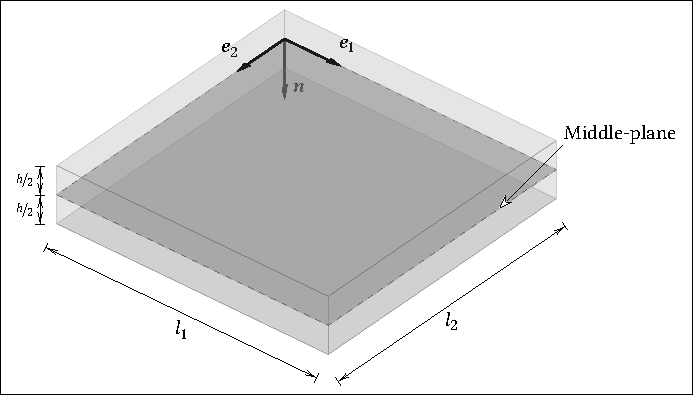
\includegraphics[scale=1]{typical_plate.pdf}
\caption{A typical plate and its middle-plane}\label{fig:generalplate}
\end{figure}

	\paragraph{Selecting a theory} Selecting the proper plate theory, among the classic ones, requires addressing two consideration~\autocite{Birman.2011}:
	\begin{enumerate}
		\item Thickness of the plate ($h$) and its transverse shear stiffness: thick plates with low transverse shear stiffness are best described by shear-deformable theories. The thinness of a plate is defined by empirical measures, e.g., a thickness less than one-tenth of its smallest dimension is considered thin $h<0.1\text{min}(l_1,l_2)$~\autocite{Altenbach.2008} or more restrictive values such as $h<0.05\text{min}(l_1,l_2)$~\autocite{Ugural.2010}. 
		\item Geometrical linearity or non-linearity of the problem: it is determined by the relative magnitude of deflection ($w$) to plate thickness. Namely, non-linearity is negligible for `small' deformations, i.e., deflections smaller than the empirical values of ($w<0.5h$)~\autocite{Birman.2011} or ($w<0.2h$)~\autocite{Altenbach.2008}. 
	\end{enumerate}
	In the absence of the shear strain components, deformation of the thin plate is dominated by bending. However, the effect of shear should be considered through some correction factors in special cases, e.g., plates with holes~\autocite{Timoshenko.1959}.

The adopted criterion of linearity assures the applicability of the small-deflection models in which the Green-Lagrange strain tensor reduces to the linearised strain measure because of the negligible quadratic slope terms. The other consequence of small deformations is that the middle-plane does not strain and becomes the neutral plane.

\paragraph{Plate categories} Note that the overlap of geometrical non-linearity and shear deformability is not common except for the case of sandwich panels with a very soft core. Therefore, based on the two aforementioned aspect, three categories of plates are recognised:
\begin{enumerate}
\item thin plates with small deformations,
\item thin plates with large deformations, and
\item thick plates.
\end{enumerate}









% ──────────────────────────────────────────────────────────────────────────────────────────────────
\subsection{Shear-Rigid Plate Theory}
The classic small-deformation thin plate theory is an extension of the Euler-Bernoulli beam theory. The theory ignores geometrical non-linearity and it is based on the Kirchhoff-Love hypotheses~\autocite{Reddy.2006}, which assume that the transverse normals\,\footnote{Transverse normals are the straight lines that are perpendicular to the middle-surface.} 
\begin{itemize}
\item remain straight after deformation,
\item are rigid, and
\item remain perpendicular to the middle-surface after deformation.
\end{itemize}
These assumptions have the following implications:
\begin{itemize}
\item Having `straight transverse normals after deformation' results in a linear distribution of strains through the cross-section. Thus, the middle-plane and the neutral plane coincide. In contrast, in the case of large deformations of a thin plate, the middle-plane is also strained. 
\item Due to the rigidity of the transverse normals, the thickness of the plate remains constant, i.e., no normal strains perpendicular to the neutral plane exists ($\varepsilon_{33}=0$). Consequently, the deflection of the plate becomes independent of the normal coordinate. Additionally, the normal transverse stress is usually ignored and does not enter the equilibrium equations since it is usually one order of magnitude smaller than transverse shear stresses ($\sigma_{33}\approx 0$). Thus, plane stress and constant thickness conditions are consequences of the current restriction.
\item `Transverse normals remaining perpendicular' indicates that shear deformability is neglected, i.e., the transverse shear strains ($\varepsilon_{13}$ and $\varepsilon_{23}$) are negligible. Note that although transverse shear strains are ignored, the internal transverse shear forces are obtained from the equilibrium conditions.
\end{itemize}
The Kirchhoff-Love assumptions form the shear-rigid plate theory, which is suitable for thin plates or plates with high transverse shear stiffness. 

% ──────────────────────────────────────────────────────────────────────────────────────────────────
\subsection{Shear-Deformable Plate Theory}
The shear deformable plate theory is an improvement to the shear-rigid plate theory by considering the shear strain deformations since the latter theory underestimates the deflections in thick plates. Also from another point of view, the theory is an extension of the Timoshenko beam theory to plates. 

The shear deformable theory is developed in different orders, which determine how the rotations of transverse normals are related to planar displacements. For instance, releasing the perpendicularity restriction of transverse normals results in the first-order shear deformable plate theory, i.e., additional rotations of the transverse normals due to shear strains are linearly related to each other. Releasing the straightness restriction of the transverse normals results in the third-order shear deformable theory, i.e., straight cross sections may become cubic curves after deformation~\autocite{Reddy.2006}.


\section{Laminate/Sandwich Theories}
	In terms of composite laminates and sandwiches, two main approaches exist:
	\begin{enumerate}
	\item The \textit{equivalent single-layer theories} (ESLTs)~\autocite{Altenbach.2010c} adopt the derived approach to transform the 3D problem into an equivalent 2D one. The assumptions are continuity of the displacements and/or strains through thickness. Two famous ESLTs are the classic laminate theory (CLT) (demands C\textsuperscript{1}-continuity) and first-order shear deformation theory (FSDT) (demands C\textsuperscript{0}-continuity); the former is used for thin laminates whereas the latter is used for thicker laminates and sandwiches.
	\item The \textit{layer-wise theories} (LWTs) require only C\textsuperscript{0}-continuity of through-thickness displacement but could be kinematically more accurate by incorporating layer-wise transverse shear effect into the displacement field~\autocite{Altenbach.2010c}. They could result in effortless FE implementations, see~\autocite{Javanbakht.2019b}.
	\end{enumerate}
	Among the ESLTs, the CLT is discussed in the sequel.

\paragraph{Assumptions of CLT} Classic laminate theory is merely the extension of thin plate theory to accommodate laminates. It is based upon the following assumption~\autocite{Herakovich.1998}:
    \begin{enumerate}
        \item perfect inter-layer bonding exists,
        \item each layer is homogeneous and can be orthotropic, transversely isotropic, or isotropic,
        \item each layer is in the plane stress state\,\footnote{In plane stress state, there exists a strain perpendicular to the plane of stress due to Poisson's effect, which will be ignored in the current context. Namely, no thickness change will be considered in CLT.}, and
        \item the laminate deforms according to shear-rigid theory.
    \end{enumerate}



\paragraph{Stress and Moment-Stress Resultants}	Consider the coordinate system in Fig.~\ref{fig:internal_force} that is established on the middle-plane of a plate (or equivalently a ply of a laminate). The basis vectors of $\base_1,\base_2$ and $\tena{n}$ are selected in a way that $\tena{n}$ is perpendicular to the middle plane; the respective coordinates are $X_1,X_2$ and $X_3$. Thereby, the Cauchy stress tensor is decomposed into	
	\begin{equation}
	\tenb{\sigma}=\sigma_{\alpha\beta}\base_\alpha\dyad\base_\beta+\sigma_{\alpha 3}\base_\alpha\dyad\tena{n}+\sigma_{3 \alpha}\tena{n}\dyad\base_\alpha+\sigma_{33}\tena{n}\dyad\tena{n},
	\end{equation}
	where the Greek indices vary from 1 to 2. 
\begin{figure}[!h]
\centering
\subfloat[Membrane and shear force resultants]{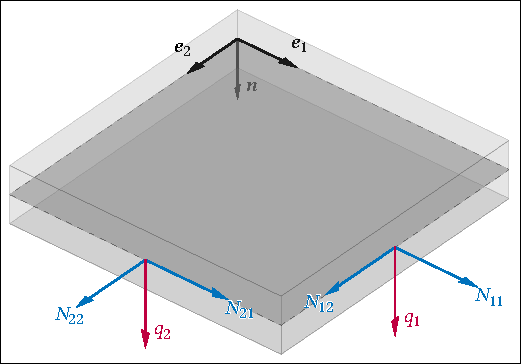
\includegraphics[scale=1]{plate_membrane_shear.pdf}}\\
\subfloat[Bending and twisting moment resultants]{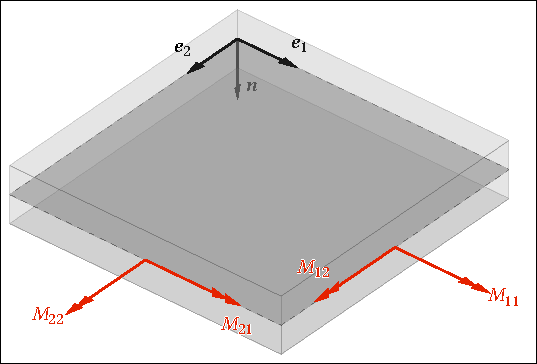
\includegraphics[scale=1]{plate_moment.pdf}}
\caption{Internal forces in a plate denoted at their positive direction}
\label{fig:internal_force}
\end{figure}%	
	If the first fundamental tensor of the surface ($\tenb{A}\equidef\tena{n}\dyad\tena{n}$)~\autocite{Eremeyev.2013} is used as a projection tensor, the 3D stress tensor could be readily projected onto the $1$-$2$ plane to form a non-symmetrical stress tensor:
	\begin{equation}
	\tenb{A}\scp\tenb{\sigma}=\sigma_{\alpha\beta}\base_\alpha\dyad\base_\beta+\sigma_{\alpha 3}\base_\alpha\dyad\tena{n},
	\end{equation}
	where $\tenb{A}\scp\tenb{\sigma}$ holds the membrane stress components $\sigma_{\alpha\beta}$ and transverse shear stress components $\sigma_{\alpha 3}$. Thereby, all the stress components on the surface with the normal of $\tena{n}$ are discarded. Now, the distribution of other stress components through thickness must by taken into account and then eliminated. To this end, the through-thickness integration operator is defined as
	\begin{equation}
	\inbrack{\Box}\equiv\thickint{\Box},
	\end{equation}
	where a structural thickness of $h$ is assumed for a plate with a normal along the 3-axis. Applying this operator to the non-symmetrical stress tensor results in
	\begin{equation}
	\inbrack{\tenb{A}\scp\tenb{\sigma}}=\tenb{N}+\tena{q}\dyad\tena{n},
	\end{equation}
	where $\tenb{N}\equiv \tenb{A}\Rayleigh\tenb{\sigma}=\inbrack{\sigma_{\alpha\beta}\base_\alpha\dyad\base_\beta}$ is the membrane stress resultant tensor and $\tena{q}=\inbrack{\sigma_{\alpha 3}\base_\alpha}$ is the transverse shear stress resultant vector. 
	
	Furthermore, the axial (bending/twisting) moment tensor, resulting from the membrane stresses, is defined as
	\begin{equation}
	\tenb{M}\equidef \inbrack{-X_3 \sigma_{\alpha\beta}\base_\alpha\dyad\base_\beta\cross\tena{n}},
	\end{equation}
	which could be replaced by its polar counterpart by removing the axial property of its second index
	\begin{equation}
	\tenb{L}\equidef \tenb{M}\cross \tena{n} = X_3 \sigma_{\alpha\beta}\base_\alpha\dyad\base_\beta,
	\end{equation}
	where $\tenb{L}$ is the polar (bending/twisting) moment tensor. 
	
	The calculated stress and moment resultants were for a single plate or ply; it can be extended to the case of a laminate structure. Namely, all the equations will be correct for each ply separately. In the CLT, the sum of these values will be used to obtain the equivalent single layer. In the following, the tensor notation will change to matrix Voigt notation, which is the common one for CLT. Namely, the stress and moment stress resultants become
	\begin{align}
		\col{N}&=\lfloor N_{11}\;N_{22}\;N_{12}\rfloor^\tran=\lfloor N_{1}\;N_{2}\;N_{6}\rfloor^\tran,\\
		\col{q}&=\lfloor q_{1}\;q_{2}\rfloor^\tran,\\
		\col{M}&=\lfloor M_{11}\;M_{22}\;M_{12}\rfloor^\tran=\lfloor M_{1}\;M_{2}\;M_{6}\rfloor^\tran,
	\end{align}
	in Voigt notation.

\paragraph{Kinematics} 	The strains of the middle-plane ($\{\mbfsansepsilon\}$) are related to the through-thickness strain field by
	\begin{equation}
	 \{\mbfsansvarepsilon(X_1,X_2,X_3)\}	= \{\mbfsansepsilon (X_1,X_2)\}+X_3\{\mbfsanskappa(X_1,X_2)\},
	\end{equation}
	 where $\symbf{\col{\mbfsanskappa}}=\lfloor \kappa_{11}\;\kappa_{22}\;\kappa_{12} \rfloor^\tran$ is the vector of bending/twisting curvature, $X_3\symbf{\col{\mbfsanskappa}}$ is the vector of flexural strains, and $\col{\mbfsansepsilon}$ is the vector of membrane (in-plane) strains. Note that since the curvature is constant through thickness (a consequence of the first assumption), the contribution of the flexural strain is linear with respect to the third coordinate. The membrane strains are also constant through thickness.


\paragraph{Resultants in laminates} For a laminate with $n$ arbitrarily-oriented plies, the overall thickness of the laminate is
\begin{equation}
	h=\sum_{k=1}^{n} h^{(k)},
\end{equation}
where $h^{(k)}$ is the thickness of the $k$-th ply from the middle-plane; namely:
\begin{equation}
	h^{(k)}=X_3^{(k)}-X_3^{(k-1)},\qquad\forall k\in\{1,2,\ldots,n\},
\end{equation}
where $X_3^{(k)}$ is the furthest distance of the $k$-th ply from the middle-plane along the normal $\tena{n}$.

The total in-plane stress resultant force vector $\col{N}$, total transverse shear resultants $\col{q}$ and the total moment-stress resultant vector $\col{M}$ of the laminate is
\begin{subequations}
\begin{align}
	\col{N}&= \sum_{k=1}^{n} \{{\symbfsf N}^{(k)}\},\\
	\col{q}&= \sum_{k=1}^{n} \{{\symbfsf q}^{(k)}\},\\
	\col{M}&= \sum_{k=1}^{n} \{{\symbfsf M}^{(k)}\},
\end{align}
\end{subequations}
	where $\{{\symbfsf N}^{(k)}\}$, $\{{\symbfsf q}^{(k)}\}$ and $\{{\symbfsf M}^{(k)}\}$ are the in-plane stress, transverse shear stress, and moment-stress resultant vector of the $k$-th ply, respectively. It can be shown that the transverse shear resultant does not couple with the other two resultants, and thus the interactions of the flexural and in-plane states read
\begin{equation}
	\left[
	\begin{array}{c}
		\col{N}\\\hline
		\col{M}
	\end{array}
	\right]
	=
	\left[
		\begin{array}{@{}c|c@{}}
			\mat{A}& \mat{B}\\\hline
			\mat{B}& \mat{D}\\
		\end{array}
	\right]
	\left[
	\begin{array}{c}
		\symbf{\col{\mbfitsansepsilon}}\\\hline
		\symbf{\col{\mbfitsanskappa}}
	\end{array}
	\right],
\end{equation}	
where $\mat{A},\mat{B}$, and $\mat{D}$ are the extensional, coupling, and bending stiffness sub-matrices, respectively. The transverse shear resultant is related to the shear strain vector $\col{\mbfitsansgamma^\text{\normalfont s}}$ by
\begin{equation}
	\col{q}=\symbf{\mat{A^\text{\normalfont s}}} \col{\mbfitsansgamma^\text{\normalfont s}},
\end{equation}
where $\symbf{\mat{A^\text{\normalfont s}}}$ is the transverse shear stiffness matrix. The contribution of each layer to the total stiffness matrices is
\begin{alignat}{3}
\mat{A}&=&                              \sum_{k=1}^{n}& \left[{\tilde{\symbfsf C}}^{(k)}\right] \left(X_3^{(k)}- X_3^{(k-1)}\right),\\
\mat{B}&=&                   \frac{1}{2}\sum_{k=1}^{n}& \left[{\tilde{\symbfsf C}}^{(k)}\right] \left( (X_3^{(k)})^2- (X_3^{(k-1)})^2\right),\\
\mat{D}&=&                   \frac{1}{3}\sum_{k=1}^{n}& \left[{\tilde{\symbfsf C}}^{(k)}\right] \left( (X_3^{(k)})^3- (X_3^{(k-1)})^3\right),\\
\symbf{\mat{A^\text{\normalfont s}}} &=&\sum_{k=1}^{n}& \left[{\symbfsf C}^{(k)}\right] \left(X_3^{(k)}- X_3^{(k-1)}\right),
\end{alignat}
where $\left[{\symbfsf C}^{(k)}\right]$ is the stiffness matrix of the $k$-th layer and $\left[{\tilde{\symbfsf C}}^{(k)}\right]$ is the reduced stiffness matrix of the $k$-th layer, see~\autocite{Altenbach.2010c,Herakovich.1998,Barbero.2017}.



%
%
%% ══════════════════════════════════════════════════════════════════════════════════════════════════
%\section{The Direct Approach}
%    In the following sections, a 3D continuum is reformulated as a 2D surface by means of the direct approach. Although no exact 2D~shell theory exists, a 2D~surface is a facilitative vehicle for mathematical formulation. Thus, the direct approach takes the 2D~surface as a primitive concept while denying it as a 3D~entity~\autocite{Libai.2005}. Aligned with this approach, simple shells are considered as 2D continua in which the interaction of the body sections is done via forces and moments~\autocite{Zhilin.1976}. 
%    
%    Herein, the so-called direct approach is used to obtain the theory for simple shells. This approach takes advantage of the fact that the directed deformable surfaces inherently have the same DoFs as those required in the shell theories. In the common shell theories of the Cauchy continua, translational DoFs are used along with some assumptions to obtain the kinematics of the problem whereas the directed surface theory has all the required kinematic quantities. Namely, all the ingredients of a shell theory, i.e., rotations and translations, are already incorporated in the directed surface effortlessly. Therefore, an assumption-free approach can be adopted.
%
%    Media with micro-structure deviate from the classical local theories and are represented using one of the 3M continua, i.e., micromorphic, microstretch, or micropolar continua with 9, 4, and 3 additional DoFs, respectively~\autocite{Eringen.1998}. The additional DoFs are assigned to each point by means of a triad of vectors---called \textit{directors}---which capture the microdeformations of the internal structure.
%
%    The most general micromorphic continuum uses deformable directors to incorporate point-wise shear, stretch, and rotations. In microstretch continuum microshearing is not possible but rotations and stretches are allowed. Finally, the micropolar continua assigns only rotations via rigid directors. Following this hierarchy, the classical Cauchy continuum is the one without any directors, i.e., it is not a directed medium. 
%    
%    Among the 3M~media, the micropolar continua have the required additional rotations, and thus it is the starting point of the direct approach. Due to the in-plane rigidity of shells, only two rotations out of the available three rotations are practically necessary. Namely, the rotations about the normal vector of the shell are neglected resulting in the so-called \textit{5-DoF theories}.
%    
%\subsection{Kinematics}
%In the 5-DoF Mindlin plate theory, three translations and two rotations are present. Zhilin \autocite*{Zhilin.1976} introduces the following DoFs: 
%\begin{alignat}{2}
%&\tena{u}   &&=u_i\base_i,\\
%&\tena{\psi}&&=\psi_\alpha\base_\alpha=-\varphi_2\base_1+\varphi_1\base_2,
%\end{alignat}
%whereas Pal'mov's \autocite*{Palmov.1982} alternative DoFs result in a better symmetry in the numerical solution:
%\begin{alignat}{3}
%&\tena{u}&&=\tena{v}+w\tena{n}&&\hspace*{2cm}\text{with}\,\tena{v}=v_\alpha\tena{e}_\alpha\;,\\
%&\tena{\varphi}&&=\varphi_\alpha\tena{e}_\alpha\;,&&
%\end{alignat}
%where $\tena{u}$ is the displacement vector, $\tena{v}$ is the in-plane displacement vector, $w\tena{n}$ is the deflection vector, and $\tena{\varphi}$ is the out-of-plane rotation vector.
%
%\subsection{Strain Measures}
%
%
%
%
%% ══════════════════════════════════════════════════════════════════════════════════════════════════
%\section{Formulation of The Equilibrium Equations}
%
%
%
%\subsection{General 3D Micropolar Continua}
%In micropolar media, linear momentum ($\tena{\symbfscr{l}}$) and angular momentum ($\tena{\symbfscr{m}}$) of a volumetric part of the whole body ($\Part\subseteq\Body$) are respectively defined as
%\begin{alignat}{1}
%\tena{\symbfscr{l}}&\equidef\iiint_{\Part}\rho\tena{v}\dif V\\
%\tena{\symbfscr{m}}&\equidef\iiint_{\Part}\big[(\tena{r}-\tena{r}_0)\cross\rho\tena{v}+j\tena{\omega}\big]\,\dif V,
%\end{alignat}
%where $\tena{v}$ is the velocity field, $\tena{r}$ is the position vector, $\tena{r}_0$ is the position vector with respect to an arbitrary reference point, $j$ is the moment of inertia of the microparticles, and $\tena{\omega}$ is the angular velocity field. Euler's first and second laws of motion state the balance law for the linear momentum and angular momentum of a dynamic body, respectively. Namely, for a body under external force, the rates of change of linear momentum and the angular momentum about a point are equal to the total force acting on the body and the total moment acting on the body about the same point, respectively. Consequently, in a body without any external stimuli, both linear and angular momentums are conserved. Euler's laws of motion for an oriented medium are
%\begin{alignat}{3}
%\tena{\symbfscr{p}}&\equidef{\dif \tena{\symbfscr{l}} \over \dif t}&&\equimust \iiint_{\Part}\rho\tena{b}\,\dif V                                       &&+\oiint_{\partial\Part}\tena{t}\,\dif A\\
%\tena{\symbfscr{c}}&\equidef{\dif \tena{\symbfscr{m}} \over \dif t}&&\equimust \iiint_{\Part}\big[(\tena{r}-\tena{r}_0)\cross\rho\tena{f}+\rho\tena{l}\big]\,\dif V&&+\oiint_{\partial\Part}\big[(\tena{r}-\tena{r}_0)\cross\tena{t}+\tena{\mu}\big]\,\dif A,
%\end{alignat}
%where $\rho$ is the mass density, $\tena{t}$ is the stress vector (contact force per unit area), $\tena{\mu}$ is the couple stress vector (contact couple per unit area), $\tena{b}$ is the body force vector (per unit mass), and $\tena{l}$ is the body couple vector (per unit mass). Applying the Gauss-Ostrogradsky theorem to these equations results in the local form of Euler's equations of motion:
%\begin{alignat}{3}
%\diver{\tenb{T}}  &+\rho \tena{b}&                 &=\rho{\dif \tena{v}\over\dif \tena{t}},\\
% \diver{\tenb{\mu}}&+\rho \tena{l}&\;+\,\gibbs{\tenb{T}}&=j{\dif\tena{\omega}\over\dif t}.
%\end{alignat}
%Note that only Euler's first law of motion (in either global or local forms) is identical for both Cauchy and oriented media. In 3D micropolar continua, Euler's equations of motion in the absence of inertia forces are described in the local form as
%\begin{alignat}{2}
%\label{eq:lm} \diver{\tenb{T}}  &+\rho \tena{b}&                 &=\tena{0},\\
%\label{eq:am} \diver{\tenb{\mu}}&+\rho \tena{l}&\;+\,\gibbs{\tenb{T}}&=\tena{0}.
%\end{alignat}
%% ──────────────────────────────────────────────────────────────────────────────────────────────────
%\subsection{Reduction to Planar Continua}
%Herein, a flat shell on the $1$-$2$ plane is formulated from a 3D continuum. The closed surface of the 3D body volume ($\Surface\equiv\partial\Volume$) is divided into two subsets: the kinematic boundary conditions are applied on the first one ($\Surface_u$) and the static boundary conditions are applied on the remaining part ($\Surface-\Surface_\text{u}=\Surface_\text{t}$):
%\begin{subequations}
%\begin{alignat}{3}
%&\Surface_\text{u}&:\quad&&                    \tena{u}&=\tena{u}_0,\\
%                       &&&&                    \tena{\varphi}&=\tena{\varphi}_0,\\
%&\Surface_\text{t}&:\quad&& \tena{n} \scp \tenb{T}     &=\tena{f}_0,\\
%&                 &      && \tena{n} \scp \tenb{\mu}   &=\tena{m}_0.
%\end{alignat}
%\end{subequations}

%% ══════════════════════════════════════════════════════════════════════════════════════════════════
%\section{Thermal Effects on a Single Mindlin Plate}
%The thermal effects are considered through the following assumptions:
%\begin{enumerate}
%\item Mindlin plate assumption forces a plain stress state for the plate, and therefore thermal thickness changes are ignored,
%\item material properties, e.g., elastic modulus, shear modulus, Poisson's ratio and the coefficient of thermal expansion, are temperature-independent, and thus the neutral surface coincides with the middle-plane of the plate~\autocite{Mansfield.1989},
%\item the effect of heat flux through the plate can be implicitly considered as through-thickness temperature change by adopting a smooth spatial thermal field ($T\equiv T(X_1,X_2,X_3)$); herein, the through-thickness temperature change is ignored ($T\equiv T(X_1,X_2)$),
%\item geometrically nonlinear terms are ignored in measuring the strains, and
%\item the plate is considered to be isotropic and homogeneous, i.e., $\alpha_1=\alpha_2=\alpha$ and $\alpha_{12}=0$, and thus no membrane shear deformation is induced in the plate due to the temperature field.
%\end{enumerate}
%
%% Considering a through-thickness temperature variation:
%% \begin{alignat}{8}
%% &\tenb{N}^\theta=2B\inangle{\alpha\Delta\theta}\tenb{P},\\
%% &\tenb{L}^\theta=2B\inangle{\alpha\Delta\theta X_3}\tenb{P}.
%% \end{alignat}
%% Herein, a uniform through-thickness temperature is assumed.
%%───────────────────────────────────────────────────────────────────────────────────────────────────
%\subsection{Kinematics}
%In the 5-DoF Mindlin plate theory, three translations and two rotations are present. Zhilin \autocite*{Zhilin.1976} introduces the following DoFs: 
%\begin{alignat}{2}
%&\tena{u}   &&=u_i\base_i,\\
%&\tena{\psi}&&=\psi_\alpha\base_\alpha=-\varphi_2\base_1+\varphi_1\base_2,
%\end{alignat}
%whereas Pal'mov's \autocite*{Palmov.1982} alternative DoFs result in a better symmetry in the numerical solution:
%\begin{alignat}{3}
%&\tena{u}&&=\tena{v}+w\tena{n}&&\hspace*{2cm}\text{with}\,\tena{v}=v_\alpha\tena{e}_\alpha\;,\\
%&\tena{\varphi}&&=\varphi_\alpha\tena{e}_\alpha\;,&&
%\end{alignat}
%where $\tena{u}$ is the displacement vector, $\tena{v}$ is the in-plane displacement vector, $w\tena{n}$ is the deflection vector, and $\tena{\varphi}$ is the out-of-plane rotation vector.
%
%The existing eigenstrains and eigenstresses in the material are additively decomposed to thermal ($\op^\muptheta$) and residual ($\op^0$) components. Therefore, considering the Duhamel-Neumann analogy, the total strain is
%\begin{equation}
%\tenb{E}^{\mupSigma}=\tenb{E}+\tenb{E}^\muptheta+\tenb{E}^0,\label{eq:eignestrain}
%\end{equation}
%where $\tenb{E}$ is the tensor of elastic strain. Note that the compatibility condition of the strains is enforced via
%\begin{equation}
%\tenb{E}^{\mupSigma}=\gradsym{\tena{u}}.\label{eq:compat}
%\end{equation}
%The strains can be decoupled in terms of membrane strains ($\tenb{G}$), curvature changes ($\tenb{K}$), and transverse shear strains ($\tenb{g}$) according to the first-order shear deformable plate theory:
%\begin{equation}
%\tenb{E}^{\mupSigma}=\tenb{G}^{\mupSigma}+X_3\tenb{K}^{\mupSigma}+{1\over 2}\tena{g}^{\mupSigma}\dyad\tena{n}.
%\end{equation}
%Thus, the compatibility condition Eq.~\eqref{eq:compat} can be rewritten in the form of
%\begin{alignat}{3}
%\tenb{G}^{\mupSigma}&=\gradsym{\tena{v}},\\
%\tenb{K}^{\mupSigma}&=\gradsym{\tena{\varphi}},\\
%\tenb{g}^{\mupSigma}&=\grad{w}+\tena{\varphi}.
%\end{alignat}
%Similar to Eq.~\eqref{eq:eignestrain}, the decoupled strain measures can be expressed as
%\begin{alignat}{5}
%\tenb{G}^{\mupSigma}&=\tenb{G}&&+\tenb{G}^\muptheta&&+&\tenb{G}^0,\\
%\tenb{K}^{\mupSigma}&=\tenb{K}&&+\nulla            &&+&\tenb{K}^0,\\
%\tena{g}^{\mupSigma}&=\tena{g}&&+\nulla            &&+&\tena{g}^0,
%\end{alignat}
%where the decoupled thermal strains are
%\begin{alignat}{5}
%\tenb{G}^{\muptheta}&=\alpha\Delta\theta\tenb{P},\\
%\tenb{K}^{\muptheta}&=\nulla,\\%{\alpha\Delta\theta \over X_3}\tenb{P}={1\over X_3}\tenb{G}^{\muptheta},\\
%\tena{g}^{\muptheta}&=\nulla.
%\end{alignat}
%
%
%%───────────────────────────────────────────────────────────────────────────────────────────────────
%\subsection{Constitutive Law}
%Based on the Duhamel-Neumann analogy, the total stress is
%\begin{equation}
%\tenb{T}^{\mupSigma}=\tenb{T}-\tenb{T}^\muptheta-\tenb{T}^0,\label{eq:strs}
%\end{equation}
%where $\tenb{T}$ is the elastic stress tensor. However, the thermal eigenstresses will be present only in the case of incompatible thermal eigenstrains, e.g., in non-uniform temperature changes through thickness, when the material is anisotropic, or in the presence of constraints. In the case of non-zero uniform thermal strains, the respective thermal stresses are obtained from
%\begin{equation}
%\tenb{T}^{\muptheta}\!=3K\tenb{E}^\muptheta,
%\end{equation}
%where $K={3(1-2\nu) \over Y}$ is the bulk modulus. Herein, it is assumed that a homogeneous thermal field is applied, and thus $\tenb{T}^\muptheta=\tenb{0}$ and $\tenb{E}^\muptheta\neq\tenb{0}$ gives
%\begin{equation}
%\tenb{T}^{\mupSigma}=\tenb{T}-\tenb{T}^0.\label{eq:eigenstress}
%\end{equation}
%Consequently, the thermal effect is considered only via the thermal eigenstrains without any thermal eigenstresses. On the other hand, both of the residual (initial) eigenstresses and eigenstrains are taken into account, cf.~Eqs.~\eqref{eq:eignestrain} and \eqref{eq:strs}.\\
%Applying the over-thickness integration operator to Eq.~\eqref{eq:eigenstress} results in 
%\begin{equation}
%N_{\alpha\beta}=\inangle{T_{\alpha\beta}}\rightarrow \tenb{N}^{\mupSigma}=\tenb{N}-\tenb{N}^0,
%\end{equation}
%where $\tenb{N}$ is the membrane force tensor. Multiplying this equation by $X_3$ and applying the same operator results in
%\begin{equation}
%\tenb{L}^{\mupSigma}=\tenb{L}-\tenb{L}^0,
%\end{equation}
%where $\tenb{L}$ denotes the polar (bending/twisting) moment tensor.\\
%The 3D constitutive equation is expressed as~\autocite{Mura.1982}:
%\begin{equation}
%\tenb{T}^{\mupSigma}=\tend{C}\dscp \tenb{E},
%\end{equation}
%which is combined with Eqs.~\eqref{eq:eigenstress} and \eqref{eq:eignestrain} resulting in the generalised form of Duhamel-Neumann law:
%\begin{equation}
%\tenb{T}=\tend{C}\dscp(\tenb{E}^\mupSigma-\tenb{E}^\muptheta-\tenb{E}^0)+\tenb{T}^0.
%\end{equation}
%%───────────────────────────────────────────────────────────────────────────────────────────────────
%\subsection{Balance Equations}
%
%
%
%
%
%
%Since eigenstresses are already in-balance internally, the local form of the principle of balance of linear momentum (Cauchy's equation) can be readily stated in terms of elastic stresses:
%\begin{equation}
%\diver{\tenb{T}}+\rho \tena{b}=\tena{0}.
%\end{equation}
%The external distributed force vector ($\tena{f}$) is composed of two components
%\begin{alignat}{4}
%&\tena{f}=\tena{s}+\tena{q},&\qquad\text{with}\quad& \tena{s}=-s_\alpha\base_\alpha,\quad \tena{q}=q\tena{n},
%\end{alignat}
%where $\tena{s}$ is the tangential distributed external force vector, and $\tena{q}$ is the normally distributed force vector.
%
%
%In the absence of inertia forces, the balance of linear and angular momentum for micropolar media are stated as
%\begin{alignat}{3}
%\div{a}
%\end{alignat}
%
%
%
%
%
%
%
%
%
%
%
%
%
%
%
%
%
%
%%───────────────────────────────────────────────────────────────────────────────────────────────────
%\subsection{Decoupled Kinetic Measures}
%Analogous to Eq.~\eqref{eq:eigenstress}, through-thickness integration of stress tensor results in
%\begin{subequations}
%\begin{alignat}{4}
%&\tenb{N}^{\mupSigma}&&=\tenb{N}&-&\tenb{N}^\muptheta&-&\tenb{N}^0,\\\label{eq:membrane}
%&\tenb{L}^{\mupSigma}&&=\tenb{L}&-&\tenb{L}^\muptheta&-&\tenb{L}^0,\\
%&\tena{q}^{\mupSigma}&&=\tena{q}&-&\nulla            &-&\tena{q}^0,
%\end{alignat}
%\end{subequations}
%where $\tenb{N}$ is the membrane stress resultant tensor, $\tenb{L}$ is the moments resultant  tensor, and $\tena{q}$ is the transverse shear stress resultant vector. The total membrane stress resultant is obtained by over-thickness integration of the total stress tensor:
%\begin{equation}
%\tenb{N}^{\mupSigma}=\inangle{\tena{P}\scp\tenb{T}\scp\tenb{P}},
%\end{equation}
%and results in
%\begin{align}
%\tenb{N}^{\mupSigma}=\tend{A}\dscp\tenb{G}&&\text{with}\;\tend{A}=2h\left[(B-G)\tend{P}^\vol+G\tend{P}^\sym\right].\label{eq:membranetotal}
%\end{align}
%The thermal stress resultant is obtained from
%\begin{equation}
%\tenb{N}^\muptheta=2Bh\tenb{G}^\muptheta\qquad\text{with}\quad\tenb{G}^\muptheta=\alpha\mupDelta\theta\tenb{P}.\label{eq:membranethermal}
%\end{equation}
%Thus, combining Eqs.~\eqref{eq:membrane}, \eqref{eq:membranethermal}, and \eqref{eq:membranetotal} results in the elastic components of the membrane stress resultant:
%\begin{equation}
%\tenb{N}=\tend{A}\dscp\tenb{G}+2Bh\tenb{G}^\muptheta+\tenb{N}^0.
%\end{equation}
%The total moment resultant is obtained by 
%\begin{equation}
%\tenb{L}^{\mupSigma}=\inangle{\tena{P}\scp\tenb{T}\scp\tenb{P}X_3},\label{eq:momentres}
%\end{equation}
%and results in
%\begin{align}
%\tenb{L}^{\mupSigma}=\tend{D}\dscp\tenb{K}&&\text{with}\;\tend{D}={h^3\over 6}\left[(B-G)\tend{P}^\vol +G\tend{P}^\sym\right].\label{eq:momentrestot}
%\end{align}
%The thermal moment resultant is obtained from
%\begin{align}
%\tenb{L}^\muptheta={Bh^2\over 2}\tenb{G}^\muptheta&&\text{with}\;\tenb{G}^\muptheta=\alpha\mupDelta\theta\tenb{P}.\label{eq:momentthermal}
%\end{align}
%Combining the Eqs.~\eqref{eq:momentres}, \eqref{eq:momentrestot} and \eqref{eq:momentthermal}, the elastic components of the moments resultant tensor are obtained:
%\begin{align}
%\tenb{L}=\tend{D}\dscp\tenb{K}+{Bh^2\over 2}\tenb{G}^\muptheta+\tenb{L}^0.
%\end{align}
%% ──────────────────────────────────────────────────────────────────────────────────────────────────





%---------------------------------------------------------------------------------------------------
\section{Anisotropic Failure Criteria} %TODO double check everything
	\paragraph{General mathematical form} A general failure criterion for anisotropic materials can take the following form~\autocite{Goldenblat.1966}:
	\begin{equation}\label{eq:strength_aniso}
		f\equidef \sum_{k=1}^{n}
		(\tenb{\sigma}^\tenpow{k}\odot\tenn{S}{2k})^{\alpha_k} \le 1,\qquad\qquad \alpha_k \in \Real,		
%		(\tenb{\sigma}\dscp\tenb{S})^\alpha + (\tenb{\sigma}^\tenpow{1}\contract\tend{S})^\beta +
%		(\tenb{\sigma}^\tenpow{2}\contract\tenn{S}{6})^\gamma + \ldots\le 1,\qquad\qquad \alpha, \beta, \gamma, ... \in \Real,
	\end{equation}
	where Cauchy stress tensor ($\tenb{\sigma}$), and strength tensors ($\ten{S}$) are related via the scalars ($\alpha_k$). The strength tensor is the stress tensor that is obtained upon the failure of material (the ultimate stress tensor)~\autocite{Malmeister.1969}. Strength tensors are elements of the strength/failure surface. For instance, a second-order strength tensor ($\tenb{S}\in\symset$) is geometrically represented by a surface in the six-dimensional space. Initially, some points on a failure surface are obtained via experimentations, and then by statistical analysis, a surface is obtained for a specific confidence level~\autocite{Malmeister.1969}. By choosing the appropriate scalars and the order of tensors, any failure surface can be represented mathematically by the calibration of Eq.~\eqref{eq:strength_aniso}; this is the so-called \textit{tensor method}. Some general examples are presented in the sequel.
	
	\paragraph{Tsai-Hill criterion} The extension of the Huber-Mises-Hencky criterion in isotropic materials to the orthotropic ones was carried out by Hill~\autocite{Hill.1998}. Later, the so-called Tsai-Hill Criterion is presented~\parencite{Azzi.1966}:
	\begin{equation}
		f_\text{Tsi-Hill}\equidef \left(\frac{\sigma_{11}}{S_{11}}\right)^2 + \left(\frac{\sigma_{22}}{S_{22}}\right)^2 + \left(\frac{\sigma_{12}}{S_{12}}\right)^2 - \frac{\sigma_{11}\sigma_{22}}{(S_{11})^2} \le 1,
	\end{equation}
	which is obtained by the quadratic terms of Eq.~\eqref{eq:strength_aniso}. Unlike the maximum stress criterion, no specific failure mode could be identified by this criterion.
	
	
	\paragraph{Tsai-Wu criterion} The Tsai-Wu criterion~\autocite{Tsai.1971} is a special case for which the linear and quadratic terms are used~($\alpha_1=\alpha_2=1$), i.e., the linear combination of first and second order tensors:
	\begin{equation}
		f_\text{Tsi-Wu}\equidef \tenb{\sigma}\dscp\tenb{S} + (\tenb{\sigma}\dyad\tenb{\sigma})\dscp\dscp\tenn{S}{4} =\tenb{\sigma}\dscp\tenb{S} + \tenb{\sigma}\dscp\tend{S}\dscp\tenb{\sigma}^\tran.
	\end{equation}	 



	
	\paragraph{Maximum stress criterion} In this criterion, the three axial, transverse and shear failure modes of fibre-reinforced composites are decoupled:
	\begin{alignat}{2}
		\sigma_{11} \ge S_{11},\\
		\sigma_{22} \ge S_{22},\\
		\sigma_{12} \ge S_{12}.
	\end{alignat}
	By using the maximum stress criterion in the off-axis loading of a unidirectional composite, the loading angle determines the strength and failure mode, see Fig.~\ref{fig:max_stress_crit}.
\begin{figure}[!h]
\centering
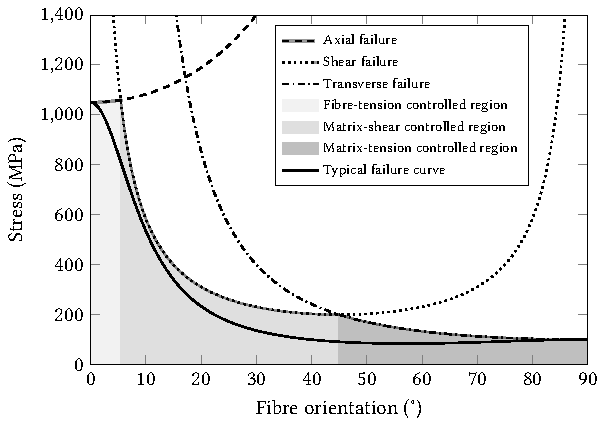
\includegraphics[scale=1]{lit_max_stress.pdf}
\caption{Dominant regions of various failure modes in a fibre-reinforced composite material due to uncoupled nature of the maximum stress criterion}\label{fig:max_stress_crit}
\end{figure}


	\paragraph{Cowin's failure criterion} 	A scalar-valued function of Cauchy stress tensor ($\tenb{\sigma}$), orientation tensor ($\tenb{H}$) and fibre volume fraction ($\zeta_\text{f}$) is assumed~\autocite{Cowin.1986}:
		\begin{equation}
			f\equiv f(\tenb{\sigma}, \tenb{H}, \zeta_\text{f}).
		\end{equation}
		Since the anisotropy of the continuum is incorporated by means of the orientation tensor, $f$ must succumb to every symmetry, i.e., it must satisfy the isotropy condition:
		\begin{equation}
			f(\tenb{\sigma}, \tenb{H}, \zeta_\text{f})\equimust f(\tenb{Q}\Rayleigh\tenb{\sigma}, \tenb{Q}\Rayleigh\tenb{H}, \zeta_\text{f}),
		\end{equation}
		where $\tenb{Q}$ is the orthogonal rotation tensor. Alternative to satisfying this equation, a form-invariant anstaz could be considered by including all the invariants of the parameters in the function~\autocite{Boehler.1987}:
		\begin{equation}
			f\equiv f\big(
			\tr{\tenb{\sigma}},\tr{\tenb{\sigma}^2},\tr{\tenb{\sigma}^3},
			\tr{\tenb{H}},\tr{\tenb{H}^2},\tr{\tenb{H}^3},
			\tr{(\tenb{\sigma}\scp\tenb{H})},\tr{(\tenb{\sigma}\scp\tenb{H}^2)},\tr{(\tenb{\sigma}^2\scp\tenb{H})},\tr{(\tenb{\sigma}^2\scp\tenb{H}^2)},\zeta_\text{f}\big).
		\end{equation}
		where $\tr{(\op)}\equidef\tenb{I}\dscp\op$ indicates the trace operator. The final result is a form of Eq.~\eqref{eq:strength_aniso} that only incorporates the linear and quadratic terms:
	\begin{equation}
		f_\text{Cowin}\equidef \tenb{\sigma}\dscp\tenb{S} + (\tenb{\sigma}\dyad\tenb{\sigma})\dscp\dscp\tend{S},
	\end{equation}	
	where the strength tensors are given as
	\begin{equation}
		\tenb{S} =\;g_1\unitb+g_2\tenb{H}+g_3\tenb{H}\scp\tenb{H},
	\end{equation}
	and
	\begin{alignat}{5}
	\nonumber 	\tend{S} =\;& \alpha_1 \unitd^\vol 
					+\alpha_2 (\tenb{H}\dyad\unitb)^\sym 
					+\alpha_3 (\tenb{H}\scp\tenb{H}\dyad\unitb)^\sym
					+\alpha_4 (\tenb{H}\dyad\tenb{H})\\\nonumber
	    			&+\alpha_5 (\tenb{H}\scp\tenb{H}\dyad\tenb{H})^\sym 
					+\alpha_6 (\tenb{H}\scp\tenb{H}\dyad\tenb{H}\scp\tenb{H})^\sym 
					+\alpha_7 \unitd^\sym\\
					&+\alpha_8 \big[(\tenb{H}\dyadu\unitb)^\sym + (\unitb\dyadu\tenb{H})^\sym\big]6
					+\alpha_9 \big[(\tenb{H}\scp\tenb{H}\dyadu\unitb)^\sym + (\unitb\dyadu\tenb{H}\scp\tenb{H})^\sym\big].
	\end{alignat}
	Note that this model requires nine parameters:
	\begin{alignat}{5}
		\alpha_i\equiv \alpha_i(\tr{\tenb{H}},\tr{\tenb{H}^2},\tr{\tenb{H}^3},\zeta_\text{f}),\qquad\qquad\forall i\in\{1,...,9\}.
	\end{alignat}		













\section{Micro-Mechanical Models}
	In this section, a background on obtaining the properties of particulate suspensions is provided. Then, the relation of such composite systems to solid-solid composites is discussed. In this regard, the classic Halpin-Tsai and Nielson models are reviewed.

\subsection{Hill Bounds \& Rule of Mixture} 
	As mentioned earlier, Cowin's formulation is used along with spectral analysis to detect the special cases. Moreover, the Hill bounds are used in developing the semi-analytical formulation of the effective properties for NFRCs. In the bounding methods of MFA, the volume averaging of an arbitrary field ($\tend{T}$) over the $\Omega$ domain is defined as
	\begin{equation}
	\avevol{\tend{T}} \equidef \int_{\Omega}\tend{T}(\tena{x})\dif\Omega,
	\end{equation}
	where $\tena{x}$ is the position vector. In a biphasic material, the domain consists of fibre (f) and matrix (m) volumes, i.e., $\Omega_\text{f} \cup \Omega_\text{m}=\Omega$ and $\Omega_\text{f} \cap \Omega_\text{m}=\varnothing$. To set up the micro-mechanical formulation for a multi-phase continuum, the micro-constitutive relation between the stress and strain of the $p$ phase is
	\begin{alignat}{2}
	\tenb{\sigma}^\text{(p)} &= \tend{C}^\text{(p)}\dscp\tenb{\varepsilon}^\text{(p)},\qquad\qquad\forall\text{p}\in\{\text{f},\text{m}\},
	\end{alignat}
	where $ \tend{C}^\text{(p)}$ is the elastic stiffness of the `p' phase. The averaged macro-constitutive relation for the homogenised medium is
	\begin{alignat}{2}
		\avevol{\tenb{\sigma}} &= \tend{C}_\text{eff}\dscp\avevol{\tenb{\varepsilon}},
	\end{alignat}
	where $\tend{C}_\text{eff}$ is the effective elastic stiffness of the multi-phase medium. The average stress and average strain of the medium are $\avevol{\tenb{\varepsilon}}=\sum\zeta^{(p)}\tenb{\varepsilon}^{(p)}$ and $\avevol{\tenb{\sigma}}	=\sum\zeta^{(p)}\tenb{\sigma}^{(p)}$ where $\zeta^{(p)}=\sfrac{\Omega_\text{p}}{\Omega}$ is the volume fraction of the `p' phase. In the next step, localisation tensors~\autocite{Hill.1963} are used to relate the overall averaged properties to the phase-averaged ones:
	\begin{alignat}{2}
	\forall\text{p}\in\{\text{f},\text{m}\}:\left\{
	\begin{array}{rl}
		\avevol{\tenb{\varepsilon}}^\text{(p)} &= \tend{A}^\text{(p)}\dscp\avevol{\tenb{\varepsilon}},\\[0.2cm]
		\avevol{\tenb{\sigma}}^\text{(p)} 	&= \tend{B}^\text{(p)}\dscp\avevol{\tenb{\sigma}}.
	\end{array}\right.,
	\end{alignat}
	where $\tend{A}$ and $\tend{B}$ are strain and stress concentration tensors, respectively.
	and obtain the effective elastic tensor
	\begin{equation}
	\tend{C}_\text{eff}=\sum_\text{(p)}\zeta^\text{(p)} \tend{A}^\text{(p)}\dscp\tend{C}^\text{(p)}.
	\end{equation}
	Adopting Voigt's assumption~\autocite{Voigt.1889} demands $ \avevol{\tenb{\varepsilon}^\text{(f)}}\equimust\avevol{\tenb{\varepsilon}^\text{(m)}}\equimust\avevol{\tenb{\varepsilon}}$ that results in the equality $\sum_\text{(p)}\zeta^{(p)}\tend{A}^\text{(p)}=\unitd^\sym$. Finally, the general form of rule of mixture for a bi-phasic medium is obtained
	\begin{equation}
	\tend{C}_\text{eff}=\sum_\text{(p)}\zeta^\text{(p)}\tend{C}^\text{(p)}.
	\end{equation}
	Adopting Reuss' assumption~\autocite{Reuss.1929} demands $ \avevol{\tenb{\sigma}^\text{(f)}}\equimust\avevol{\tenb{\sigma}^\text{(m)}}\equimust\avevol{\tenb{\sigma}}$ that results in the equality  $\sum_\text{(p)}\zeta^{(p)}\tend{B}^\text{(p)}=\unitd^\sym$. The general form of the inverse rule of mixture for a bi-phasic mediums is obtained
	\begin{equation}
	\tend{C}^\inv_\text{eff}=\sum_\text{(p)}\zeta^\text{(p)}\left(\tend{C}^\text{(p)}\right)^\inv.
	\end{equation}	
	
	 Finally, the Hill bound is obtained~\parencite{Bohm.2004}:
	\begin{equation}
		\Big[\sum_\text{(p)}\zeta^\text{(p)}(\tend{C}^\text{(p)})^\inv\Big]^\inv \le\tend{C}_\text{eff}\le\sum_\text{(p)}\zeta^\text{(p)}\tend{C}^\text{(p)},
	\end{equation}
	where $(\tend{C}^\text{(p)})^\inv$ is the compliance tensor of the phase `p'.

\paragraph{Rule of mixture} Expanding Hill's bound to their components results in the rule of mixture (RoM) and the inverse rule of mixture (IRoM):
	\begin{subequations}
	\begin{alignat}{2}
		E_\parallel 		=& \zeta_\text{f}E_\text{f}          &&+\zeta_\text{m}E_\text{m},\\
		\frac{1}{E_\perp}	=& \frac{\zeta_\text{f}}{E_\text{f}} &&+ \frac{\zeta_\text{m}}{E_\text{m}},
	\end{alignat}
	\end{subequations}
	where $\zeta$ is the volume fraction and $E$ is the elastic modulus. The subscripts `$\text{f}$' and `$\text{m}$' are used to denote the properties related to the fibres and the matrix, respectively. The elastic moduli $E_\parallel$ and $E_\perp$ are estimates in the longitudinal and transverse directions, respectively. Either formulation does not provide adequate meso-structural information regarding the composite material, and thus additional correction factors are applied to compensate this to some extent. The result is the so-called enhanced rule of mixture (En-RoM)~\autocite{Summerscales.2019}. The multiplication of the correction factors is regarded as an \textit{efficiency parameter} adjusting the contribution of fibres, see Chapters~\ref{chap:p6} and~\ref{chap:p7} for this extension.
	
\subsection{Viscosity Theory and Composite Systems}
	Viscosity is defined as the ratio of the shear stress $\tau$ to a fixed strain rate $\dot{\gamma}$---the stress is required to move a solution with a constant strain rate:
	\begin{equation}
		\eta \equidef \frac{\tau}{\dot{\gamma}(\tau)}.\label{eq:vis}
	\end{equation}
	In Newtonian fluids, viscosity does not depend on the shear rate. 
	
	In polymers, the viscosity can be used to estimate the molecular weight. Furthermore, one could calculate the effect of dissolving a solute on the viscosity of the solvent. To capture this effect, various measures of viscosity are introduced such as 
	\begin{subequations}
	\begin{alignat}{2}
		&\text{relative viscosity}\qquad& \eta_\text{r}  &\equidef \frac{\eta}{\eta_0}, \\
		&\text{specific viscosity}\qquad& \eta_\text{sp} &\equidef \frac{\eta-\eta_0}{\eta_0}, \\
		&\text{inherent viscosity}\qquad& \eta_\text{i}  &\equidef \frac{\ln\eta_\text{r}}{c}, \\
		&\text{intrinsic viscosity}\qquad& \left[\eta\right]  &\equidef \lim\limits_{c\rightarrow 0} \frac{\eta_\text{sp}}{c},
	\end{alignat}
	\end{subequations}
	where $\eta_0$ is the viscosity of the solution without the solute, $\eta$ is the viscosity of the solution with the $c$ the concentration of the solute. Relative viscosity and specific viscosity represent the change in the viscosity after dissolution in terms of final value and the change in the value, respectively. Inherent viscosity quantifies the sensitivity of the solution viscosity to change in the concentration of the solute. Intrinsic viscosity does a similar job but removes the dependency of inherent viscosity to concentration by taking a limit value. Namely, the definition of intrinsic viscosity can be set up by taking a limit value of the inherent viscosity and considering the fact that specific viscosity becomes very small at the limit:
	\begin{equation}\label{eq:spsv}
		\left[\eta\right] 
		\equidef  \lim\limits_{c\rightarrow 0} \ln \eta_\text{i}
		= \lim\limits_{c\rightarrow 0} \frac{\ln \eta_\text{r}}{c} 
		= \lim\limits_{c\rightarrow 0} \frac{\ln(1+\eta_\text{sp})}{c} 
		\approx \lim\limits_{c\rightarrow 0} \frac{\eta_\text{sp}}{c},
	\end{equation}
	in which Taylor's expansion is utilised and higher order terms are neglected. Namely, inherent and intrinsic viscosities have the same value as the concentration approaches zero. The result is a dimensionless material property which is independent of the concentration.
	Since intrinsic viscosity only depends on the molecular weight, it is the perfect tool for investigating the he effect of a solute in the viscosity of the solvent.
	
	Calculation of the intrinsic viscosity is done by calculating the specific viscosity for different concentrations and extrapolating the result to zero concentration. However, in an ideal solution\footnote{In an ideal gas, the interaction between molecules/atoms are negligible whereas in a liquid inter-molecular forces cannot be ignored. Thus, in an ideal liquid, the average inter-molecular interaction is assumed to be the same everywhere.}, the specific viscosity does not depend on concentration and taking a limit value is trivial\footnote{In ideal solutions, the inherent viscosity is obviously not equal to specific viscosity. Although specific viscosity is independent of concentration in ideal solutions, inherent viscosity will still depend on the concentration.}. In such cases, Eq.~\eqref{eq:spsv} reduces to
	\begin{equation}
		\left[\eta\right] = \frac{\eta_\text{sp}}{c},
	\end{equation}	
	and by rearranging, Einstein's equation to calculate the viscosity of a dilute suspension of rigid spherical particles is obtained:
	\begin{equation}
		\eta_\text{sol} = \eta_{\text{l}}(1+\left[\eta\right]c).\label{eq:ein}
	\end{equation}
	The theory of the viscosity of suspensions is extended to the theory of composite systems for obtaining the moduli of those systems. Similarities stem from the flow of suspensions during the manufacturing of composite materials~\autocite{Nielsen.1994}. Therefore, Eq.~\eqref{eq:ein} is restated for a composite system of particles and matrix:
	\begin{equation}
		\eta_\text{c} = \eta_{\text{m}}(1+k_\text{E}\zeta_\text{p, max}),
	\end{equation}	
	where $\eta_\text{c}$ is the viscosity of composite, $\eta_\text{m}$ is the viscosity of matrix, $\zeta_\text{p, max}$ is the maximum volume fraction possible for particles, and the intrinsic viscosity if relabelled to the so-called generalised Einstein's coefficient $k_\text{E}=2.5$.
	
	The maximum volume fraction for particles or the maximum packing fraction\footnote{This concept resembles the atomic packing factor of atoms in crystals, and thus quantifies how closely the particles can be packed.} is defined as
	\begin{equation}
		\zeta_\text{p, max}=\frac{V_\text{p, true}}{V_\text{p, apparent}},
	\end{equation}
	which is the ratio of the true volume of the particles ($V_\text{p, true}$) to the apparent volume ($V_\text{p, apparent}$). Since voids always exist between particles, the apparent volume is higher that the true volume, i.e., $\zeta_\text{p, max}<1$. For instance, cubic and hexagonal packing result in the maximum packing fractions of 0.524 and 0.78, respectively (see Table~\ref{table:apf}).

	\begin{table}[!h]
	\centering
	\caption{Maximum packing fractions. Adapted from~\autocite{Nielsen.1994}}\label{table:apf}
	\begin{tabular}{p{0.12\textwidth}p{0.6\textwidth}p{0.175\textwidth}}
	\toprule
	\bfs{Inclusion}	&	\bfs{Arrangement}	&	$\zeta_\text{p, max}$ \bfs{or} $\zeta_\text{f, max}$\\
	\toprule
	Spheres	
		& Hexagonal close packing, face-centred cubic packing	& 0.7405\\
		& Body-centred cubic									& 0.60\\
		& Simple cubic											& 0.5236\\
		& Random close packing, non-agglomerated				& 0.632\\
		& Random loose packing, non-agglomerated				& 0.601\\
		& Random close packing, agglomerated					& 0.37\\\midrule
	Fibres
		& Parallel hexagonal packing							& 0.907\\
		& Parallel random packing								& 0.85\\
		& Random orientation									& 0.52\\	
	\bottomrule
	\end{tabular}
	\end{table}
	
	Following the approach of moving from viscous solutions to composite solids, the rate of shear in Eq.~\eqref{eq:vis} is replaced by shear strain. Thus, for systems with incompressible matrices ($\nu=0.5$) like an elastomer that is filled with rigid particles, the shear moduli is theoretically related to viscosity values:
	\begin{equation}
		\frac{\eta_\text{c}}{\eta_\text{m}}=	\frac{G_\text{c}}{G_\text{m}},
	\end{equation}
	where $\eta_\text{c}$ and $\eta_\text{m}$ are the viscosity of the composite and matrix, and $G_\text{c}$ and $G_\text{m}$ are the shear modulus of the composite and matrix, respectively. Fundamentally, if a theory for viscosity of a multiple phase system exists, the same theory can be use to approximate the shear moduli~\autocite{Nielsen.1994}.
	

\subsection{The Halpin-Tsai \& Lewis-Nielsen Models}
    In order to approximate the elastic properties of composites, Halpin-Tsai generalised Kerner's approach~\autocite{Kerner.1956} that resulted in the following semi-empirical formulation~\autocite{Halpin.1976}:
    \begin{equation}
        \frac{M_\text{c}}{M_\text{m}}=\frac{1+AB\zeta_\text{f}}{1-B \zeta_\text{f}},\label{eq:HT}
    \end{equation}
    where $M_\text{c}$ is a modulus of the composite, $M_\text{m}$ is the corresponding modulus of the matrix, and $\zeta_\text{f}$ is the volume fraction of fibres. In the classic Halpin-Tsai, the RoM is used to calculate the axial modulus whereas the shear, transverse, or bulk moduli are calculated from Eq.~\eqref{eq:HT}. The parameter $A$ is related to the generalised Einstein's coefficient (intrinsic viscosity) by
   	\begin{equation}
   		A=k_\text{E}-1,
   	\end{equation}
   	and thus for rigid spheres $A$ is equal to 1.5 and for long aligned fibres it goes towards infinity. Parameter $B$ considers the relative moduli of the inclusions and matrix:
    \begin{equation}
       	B=\frac{\frac{M_\text{f}}{M_\text{m}}-1 }{\frac{M_\text{f}}{M_\text{m}}+A}.
    \end{equation}
    For high relative stiffness fibres, $B$ takes a unit value. 
    
    In order to consider the maximum packing factor of the inclusions~$V_\text{f,max}$, a further generalisation is applied by introducing the $\psi$ parameter that results in the Lewis-Nielson model~\autocite{Nielsen.1970}:
    \begin{equation}
        \frac{M_\text{c}}{M_\text{m}}=\frac{1+AB\zeta_\text{f}}{1-B\psi \zeta_\text{f}},
    \end{equation}
	where $M_\text{c}$ represents a modulus for the composite, e.g., axial, transverse, shear or bulk moduli, $M_\text{m}$ is the respective modulus of the matrix, and $\zeta_\text{f}$ is the volume fraction of fibres. One could see that substituting $\psi=1$ in the current model revives the classic Halpin-Tsai model. The $A$ and $B$ parameters are common between the two models: parameter~$B$ takes into account the property contrast between the fibre and matrix phases while the $A$~parameter considers the geometry of the inclusions (particles or fibres), packing arrangement, and loading condition~\autocite{Nielsen.1994}. For a known elastic modulus, its value can be estimated by
	\begin{equation}
		A=\frac{E_\text{f}\,(E_\text{c}-E_\text{m})-\zeta_\text{f}E_\text{c}(E_\text{f}-E_\text{m})}
		   	   {E_\text{m}(E_\text{f}-E_\text{c})-\zeta_\text{m}(E_\text{f}-E_\text{m})}.
	\end{equation}
    The $\psi$ parameter depends on the maximum packing factor of the inclusions~$\zeta_\text{f,max}$:
    \begin{equation}
	\zeta_\text{f,max}\equidef\frac{V_\text{true}}{V_\text{apparent}},
    \end{equation}
    where $V_\text{true}$ is the true volume of the particles and $V_\text{apparent}$ is the volume that they appear to occupy (bulk volume). In~\autocite{Milewski.1978}, it was shown that by increasing the aspect ratio of fibres, the bulk volume of the material increases, i.e., the apparent volume increases. Thus, one could relate $\zeta_\text{f,max}$ to the aspect ratio of fibres and obtain more refined values of $\psi$. Nevertheless, several empirical equations are provided for the calculation thereof such as
    \begin{equation}
    	\psi\equidef 1+ \frac{1-\zeta_\text{f,max}}{\zeta_\text{f,max}^2}\zeta_\text{f}.
    \end{equation}
    These equations were extended to randomly-oriented fibre-reinforced composite by proposing extended values for~$A$~\autocite{Nielsen.1994, Lewis.1970, Nielsen.1970}, see Table~\ref{table:HT}. Note that in the original Halpin-Tsai formulation, the longitudinal elastic modulus is calculated by means of the RoM, which is only applicable to long fibre composites. Other suggested values for $A$ can be found in~\autocite{Halpin.1992}. 

    \begin{table}[!h]
    \centering
    \caption{Recommended values for $A$ for generalised Halpin-Tsai equations. Adapted from~\autocite{Nielsen.1994}}\label{table:HT}
    \begin{tabular}{p{0.3\textwidth}p{0.3\textwidth}p{0.3\textwidth}}
    \toprule
    \bfs{Composite Type} & \bfs{Calculated Modulus}   &  \bfs{Value of} $A$ \\
    \toprule
    Aligned fibres					         & $E_\text{L}$  				& $\sfrac{2L}{D}$\\
                                             & $E_\text{T}$  				& $0.5$\\
                                             & $G_\text{LT}$ 				& $1.0$\\
                                             & $G_\text{TT}$ 				& $0.5$\\
                                             & $K$           				& $0$\\\midrule
    Randomly-oriented fibres				 & $G$ for $\sfrac{L}{D}=4$ 		& 2.08--3.08\\
                                             & $G$ for $\sfrac{L}{D}=6$  	& 2.84--3.84\\
                                             & $G$ for $\sfrac{L}{D}=8$  	& 3.80--4.80\\
                                             & $G$ for $\sfrac{L}{D}=10$  	& 4.93--5.93\\
                                             & $G$ for $\sfrac{L}{D}=12$  	& 6.20--7.30\\
                                             & $G$ for $\sfrac{L}{D}=15$  	& 8.38--9.38\\
                                             & $G$ for $\sfrac{L}{D}=\infty$	& $\infty$\\
    \bottomrule
    \end{tabular}
    \end{table}
    
    Once the elastic moduli for aligned fibres are obtained, the elastic modulus along any arbitrary direction with respect to fibres is obtained from the classical lamination theory~\autocite{Herakovich.1998}
    \begin{equation}
    	\frac{1}{E_\theta} = \frac{\cos^4\!\theta}{E_\text{L}} +\frac{\sin^4\!\theta}{E_\text{T}} + (\frac{1}{G_\text{LT}}-2\frac{\nu_\text{LT}}{E_\text{L}})\sin^2\!\theta\cos^2\!\theta,
    \end{equation}
    where $\theta$ is the angle between the fibres and the intended direction, and $\nu_\text{LT}=-\frac{\varepsilon_\text{T}}{\varepsilon_\text{L}}$. Obviously, the maximum elastic modulus is obtained along the fibres. Similarly, the shear modulus along any arbitrary direction is 
    \begin{equation}
    	\frac{1}{G_\theta} = \frac{1}{G_\text{L}} +
    	4\left(
    	 \frac{1+\nu_\text{LT}}{E_\text{L}}+
    	 \frac{1+\nu_\text{TL}}{E_\text{T}}-
    	 \frac{1}{G_\text{LT}}
    	\right)
    	\sin^2\!\theta\cos^2\!\theta,
    \end{equation}
    The maximum shear modulus is obtained along the direction which makes $45^\circ$ with the fibre direction, i.e., maximum shear stress is transferred to the fibres.

\subsection{Composite Cylinders/Spheres Assemblage}
	Homogenisation of the continuous fibre-reinforced composites can be done by selecting a cylindrical/spherical RVE---which results in the so-called composite cylinders assemblage (CCA), and composite spheres assemblage (CSA). These micromechanical model was first introduced in~\parencite{Hashin.1964} for evaluating the effective mechanical properties of hollow fibres within a matrix; it is a two-phase model, i.e., a self-consistent model, which needs $n$-phase models for the same number of phases. Later, the mechanical properties of two-phase composite materials were considered in~\parencite{Christensen.1979} in a three-phase model. The latter effort marks the initial steps of the generalised self-consistent approach~\parencite{Bohm.2020} in which $n$-phase materials are modelled using $(n+1)$-phase models~\parencite{Herve.1993}. 
	
	By using several concentric cylinders in the CCA model, each outer phase is modelled as a ring and the inner phase would be of a circular cross-section. Namely, the continuous fibres are replaced by a representative cross-section that implies the plain strain state for the problem. The homogenised medium would be of a circular cross-section that should admit to the boundary conditions of the original assembly. For instance in a thermal problem, the RVE and the model are linked together by enforcing the same temperature and heat flow on each of their boundaries. Originally, electrical conductivity of a two-phase composites was obtained in~\autocite{Kerner.1956b}. The same results of magnetic permeability of composite materials was obtained in~\autocite{Hashin.1962b} by means of variational principles. Later on, the interpretation of the latter manifested itself as the Hashin-Shtrikman bounds. 
	
	Herein, the CSA model is adopted and extended for a four-phase composite in the context of thermal conductivity. The CSA model is very similar to the CCA except that in the former, concentric spheres are used instead of cylinders. For a typical two-phase composite, the lower bound of the effective thermal conductivity is obtained from~\autocite{Christensen.2012}:
	\begin{equation}
	k_\text{eff}=k_2 + \frac{3p_1k_2}{p_2-3\frac{k_2}{k_2-k_1}},\label{eq:cca}
	\end{equation}
	where $k_1$ is thermal conductivity of the core, $k_2$ is the thermal conductivity of the coating; $p_1$ and $p_2$ are the volume fractions of the the core and coating, respectively. In a 3D~model the core is a sphere (radius $r_1$) within another sphere as a coating (radius $r_2$), see Fig.~\ref{fig:CCA}. Note that in analogy with composite materials, the coating is the matrix and the core is the particle. Thus, $p_1=(\sfrac{r_1}{r_2})^3$ and $p_2=1-p_1$ are readily obtained.

\begin{figure}[!h]
  \centering
  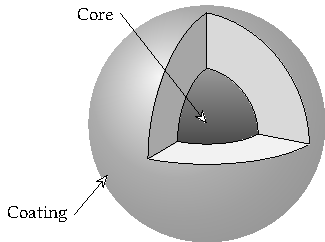
\includegraphics[scale=1]{lit_CCA}
  \caption{Schematic representation of concentric spheres of a two-phase composite}
  \label{fig:CCA}
\end{figure}
	
	It was shown that the differential equations of the CSA model (Fourier's transform law) could be used to incorporate additional phases in a spherical coordinate system~\autocite{Christensen.2012}. However, applying the continuity conditions on the interfaces and the boundary conditions on the outer surface creates a cumbersome process. By observing the repeating solutions of the differential equations in the middle rings, one could think of a recurring procedure. In~\parencite{Milton.2002}, such a procedure is introduced for particle-reinforced composites in which particle are covered with several coatings, see Fig.~\ref{fig:CCA2}. 

\begin{figure}[!h]
  \centering
  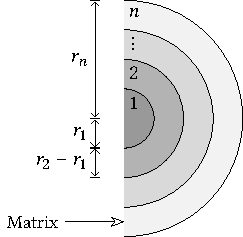
\includegraphics[scale=1]{lit_CCA2}
  \caption{A slice of several concentric hemispheres represented in 2D for multi-phase materials}
  \label{fig:CCA2}
\end{figure}	
	
	By adopting several concentric spheres (one sphere per phase), Eq.~\eqref{eq:cca} can be extended to $n$-phases:
	\begin{subequations}
	\begin{alignat}{2}
	k_{(1,2)}    &=k_2 + \frac{3p_1k_2}{p_2-\frac{3k_2}{k_2-k_1}},     \\
	k_{(1,2,3)}  &=k_3 + \frac{3p_{(1,2)}k_3}{p_2-\frac{3k_2}{k_2-k_{(1,2)}}},	\\
	k_{(1,2,3,4)}&=k_4 + \frac{3p_{(1,2,3)}k_4}{p_4-\frac{3k_4}{k_4-k_{(1,2,3)}}},	\\\nonumber
	\vdots\\
	k_{(1,2,\ldots,n)}&=k_n + \frac{3p_{( 1,2,\ldots,[n-1])}k_n}{p_n-\frac{3k_n}{k_n-k_{(1,2,\ldots,[n-1])}}}
	\end{alignat}
	\end{subequations}
	
	where $k_{(1,2,\ldots,n)}$ is the effective thermal conductivity of $n$ phases. One should notice that the number of required models/equations has reduced to $n-1$ with this method. Moreover, the fraction of each phase is defined as follows
	\begin{subequations}
	\begin{alignat}{3}
	p_{1} &= (\frac{r_1}{r_2})^3,&&&   p_{2}&=1-p{1},   \\
	p_{(1,2)} &= (\frac{r_1+r_2}{r_3})^3,&&&   p_{3}&=1-p{(1,2)},   \\
	p_{(1,2,3)} &= (\frac{r_1+r_2+r_3}{r_4})^3,&&&   p_{4}&=1-p{(1,2,3)},   \\\nonumber
	\vdots\\
	p_{(1,2,\ldots,n-1)} &= (\frac{\sum_{1}^{n-1}r_i}{r_n})^3,&&\qquad&   p_{n}&=1-p{(1,2,\ldots,n-1)},
	\end{alignat}
	\end{subequations}	
	where the last volume fraction $p_{(1,2,\ldots,n-1)}$ corresponds to the volume fraction of the reinforcements. One note that requires attention is that the outermost coating should always be the matrix.


\subsection{General Theory of Eigenstrains}
    Mura~\autocite*{Mura.1982} introduced the generic \textit{Eigenstrain} term for any stored (permanent) inelastic strains, which was inspired by Reißner's~\autocite*{Reissner.1931} classic work. The source of eigenstrains can be inhomogeneous inelastic deformations, plastic strains, creep strains, phase transformations, misfit strains, piezoelectric strains and temperature gradients among others. Thus, one great advantage of this generalization is that the all these different type of strains can be studied under one generic topic irrespective of their origin~\autocite{Jun.2010,Nyashin.2005}.

The general theory of eigenstrains deals with only two types of strains: elastic strains and eigenstrains. The main postulate of the theory is the additive decomposition of the actual strain (the total strain $\tenb{\varepsilon}^{\mupSigma}$): 
\begin{equation}
\tenb{\varepsilon}^{\mupSigma}=\tenb{\varepsilon}+\tenb{\varepsilon}^\eigen,\label{eq:eignestrains}
\end{equation}
where $\tenb{\varepsilon}$ is the elastic strain, and $\tenb{\varepsilon}^\eigen$ is the sum of all eigenstrains. Obviously, loading and unloading of an elastic stress-free body creates and removes elastic strains, respectively. Thus, eigenstrains (inelastic strains) are necessary but not enough to generate residual stresses. 

In classic continuum mechanics, the compatibility condition ensures that no overlap of the particles or gap between them happens in a continuum. The mathematical equivalent of this notion is Saint-Venant's compatibility theorem, which requires 
\begin{equation}
\curl{(\curl{\tenb{\varepsilon}})^\tran}=\nullb,\label{eq:saint}
\end{equation}
for an arbitrary tensor field $\tenb{\varepsilon}$ so that the respective displacement field $\tena{u}$ exists. The displacement field is found by solving the partial differential equation
\begin{equation}
\tenb{\varepsilon}=\gradsym{\tena{u}}.\label{eq:kinematics}
\end{equation}
In the presence of eigenstrains and by assuming a compatible elastic strain field, applying the compatibility condition to the total strain field results in
\begin{equation}
\curl{(\curl{\tenb{\varepsilon}})^\tran}=\curl{(\curl{\tenb{\varepsilon}^\eigen})^\tran}.\label{eq:sainttotal}
\end{equation}
    The right-hand side of this equation becomes non-zero for incompatible eigenstrains. By excluding the possibility of any gaps or overlaps, the incompatible eigenstrains give rise to eigenstresses. In this context, the incompatibility means that the strain field within the body cannot exist in a null stress state, i.e., an internal stress is required to enforce the strain field. This internal stress becomes present without any external force or constraints but only due to the necessity of satisfying kinematic conditions and the equilibrium equations. Such remaining internal stresses are the so-called \textit{residual stresses} in the engineering terminology, e.g., residual stresses due to fabrication and thermal stresses due to thermal expansion~\autocite{Hill.1996}. Two definitions of such residual stress is available in the literature:
\begin{enumerate}
\item Mura~\autocite*{Mura.1987} introduced a very restrictive definition: eigenstresses are self-equilibrated internal stresses, which are not caused by any external forces or constraints. Basically, any internal stress in the unloaded unconstrained body is an eigenstress.
\item Later, \citeauthor{Irschik.1988}~\autocite*{Irschik.1988} introduced the more relaxed concept of \textit{self-stress}, which is the internally equilibrated stress in the absence of external force but surface constraints are allowed.
\end{enumerate}
Herein, the first definition is adopted, and thus
\begin{equation}
\diver{\tenb{\sigma}^\eigen}=\nulla,\label{eq:eigenstressbalance}
\end{equation}
satisfies the equilibrium of the eigenstresses while
\begin{equation}
\tena{n}\scp\tenb{\sigma}^\eigen =\nulla,
\end{equation}
ensures a traction-free surface with an outward normal $\tena{n}$. 

Note that incompatible eigenstrains are the source of eigenstresses but not the other way around: incompatible eigenstrains generate elastic strains, which induce stress in the body~\autocite{Korsunsky.2017f}. The elastic strains are related to the total stress by Hooke's law:
\begin{equation}
\tenb{\sigma}^\mupSigma=\tend{C}\dscp \tenb{\varepsilon},\label{eq:eigenhooke}
\end{equation}
where $\tend{C}$ is the \textit{elastic tensor} or its inverse relation
\begin{equation}
\tenb{\varepsilon}=\tend{C}^\inv\dscp \tenb{\sigma}^\mupSigma,
\end{equation}
where $\tend{C}^\inv$ is the \textit{compliance tensor}.

In the free body condition (no external load and not constraints), the absence of eigenstrains indicates that there are no eigenstresses. In contrast, in the presence of eigenstrains, eigenstresses may or may not arise. The eigenstresses of the latter case are called \textit{impotent} or \textit{stress-free eigenstrains}, which are basically compatible or uniform strains. For instance, unconstrained uniform thermal strains are of this kind~\autocite{Korsunsky.2008}. 

\subsection{The Eshelby Method}
	The Eshelby method~\autocite{Eshelby.1957,Eshelby.1961} discusses the inclusion of ellipsoidal inhomogeneities within an infinite matrix. For the expense of incorporating an additional strain field around the inclusion, an equivalent homogeneous inclusion replaces the original inhomogeneity.\footnote{The `inhomogeneity' term implies that the inclusion is of a different material than the matrix whereas the `homogeneous' term implies that the inclusion is of the same material as the matrix. This is an interesting `thought experience'~\autocite[p.~89]{Clyne.2019} as it seems there is no justification for using the same material as of the matrix for the inclusion; mechanically there is not but mathematically there is.} Since the former has the same properties as of the matrix, the material discontinuity is thereby eliminated.
	
	Eshelby's \textit{equivalent inclusion method} takes advantage of a special impotent eigenstrain to transform the inhomogeneous inclusion to its equivalent homogeneous counterpart---the so-called `transformation strain'. To this end, the Eshelby tensor $\tenb{S}$ is introduced
	\begin{equation}
	\tenb{\varepsilon}^\text{C}=\tenb{S}\scp\tenb{\varepsilon}^\text{T},
	\end{equation}
	where $\tenb{\varepsilon}^\text{C}$ is the constrained strain and $\tenb{\varepsilon}^\text{T}$ is the transformation strain. Note that the Eshelby tensor depends only on the aspect ratio of the ellipsoidal inclusions. Once this tensor is known, the effective elastic tensor of the composites can be found~\autocite{Clyne.2019}:
	\begin{equation}
	\tend{C}_\text{eff}=\Big[(\tend{C}^\text{m})^\inv-\zeta_\text{f}\big[ (\tend{C}^\text{f}-\tend{C}^\text{m})\big(\tenb{S}-\zeta_\text{f}(\tenb{S}-\unitb)\big)+\tend{C}^\text{m}\big]^\inv(\tend{C}^\text{f}-\tend{C}^\text{m})(\tend{C}^\text{m})^\inv\Big]^\inv.
	\end{equation}
	One important assumption in this mean-field approach is that applying a far-field homogeneous strain to the composite induces a uniform strain in the inclusion~\autocite{Bohm.2020}. This implies a uniform stress for an elastic inclusion:
	\begin{subequations}
	\begin{align}
	\avevol{\tenb{\varepsilon}}^\text{(i)}&=\tenb{\varepsilon}^\text{(i)},\\
	\avevol{\tenb{\sigma}}^\text{(i)}&=\tenb{\sigma}^\text{(i)}.
	\end{align}
	\end{subequations}
	Note that this approach is valid for dilute composites. In the case of non-dilute composites, one way of taking into account the interaction of the fibres, is to introduce a background or image stress, which will be superimposed on the dilute stress field. Alternatively, the average of the disturbed strain field can be used. An analogous method is used in the following section to extend the Eshelby approach to heat transfer problems.

\subsection{The Hatta-Taya Model}
	There exist an analogy between various field values that are related by field theories. These theories usually assume a linear relationship that states the gradient of a field value is proportional to its dual; the constant of proportionality is usually a material property. From the representation theory point of view, another interpretation is possible, i.e., only the first-order terms of the generalised Taylor expansion is taken to represent the physical law. For instance in the context of elasticity, the stress is related to the gradient of deformation (strain) via the elastic tensor (Hooke's law); similarly in the heat transfer phenomenon, the gradient of temperature is related to heat flux via the thermal conductivity tensor (Fourier's law).

	Following the mentioned analogy, the Eshelby method, which was applied to obtain mechanical properties, was extended to acquire effective thermal properties in~\autocite{Hatta.1985}. Namely, the equivalent inclusion method was applied to heat transfer phenomena. Later, a similar approach was applied to coated inclusion~\autocite{Hatta.1986,Taya.1989}. In these studies, the assumption of dilute was released and the produced results remained in good agreements with the experimental ones up to 50\% fibre volume fraction as well as other method such the laminate analogy approach~\autocite{Fu.2003}. This latter approach categorises all the fibres---with the same orientation and length distributions---into a group that is modelled as a single laminate. Thus, the whole composite comprises of several laminates, i.e., a multi-directional laminar composite~\autocite{Callister.2018}. 	
	
	The Eshelby method in heat conduction establishes the equivalence between an inhomogeneity and its homogeneous counterpart by demanding the same heat flux through them.~\footnote{From a slightly different perspective, the principle of superposition can be used to additively decompose the heterogeneous media into a homogeneous problems and a deviation problem; this approach is common in Duhamel-Neumann type problems, see~\autocite{Javanbakht.2019b,Ghosh.2011,Oliver.2017}.} In non-dilute composite systems, the interaction of fibres are transferred through the matrix. In heat conduction, this is done by perturbing the temperature gradient field. Thus, the volume average of temperature gradient in the matrix ($\grad{\overline{T}}$) is selected as the disturbance measure of its respective field:
	\begin{equation}
		\grad{\overline{T}}=\int_{\text{D}-\mupOmega} \grad{T}^\text{T}-\grad{T}^0,
	\end{equation}
	where $\grad{T}^\text{T}$ is the total (actual) temperature gradient, $\grad{T}^0$ is the temperature gradient due to a uniform heat flux ($\tena{q}^0$) at infinity; and the matrix and inclusion domains are denoted by $\text{D}$ and $\mupOmega$, respectively.
	
	Similar to the transformation strain, the eigen-quantity of heat conduction is the transformation temperature gradient ($\grad{T}^*$) or sometimes called the eigen-temperature gradient~\autocite{Ghosh.2011}, which is used to set up a homogeneous domain. Analogously, an Eshelby tensor (usually called the S-tensor) for temperature gradient is also introduced:
	\begin{equation}
		\grad{T}^\text{C}=\tenb{S}\scp\grad{T}^*,
	\end{equation}
	where $\grad{T}^\text{C}$ is the constraint temperature gradient. The volume average of the transformation gradient, in 2D, is obtained from
	\begin{equation}
		\avevol{\grad{T}^*}_\mupOmega = \frac{1}{\zeta_{\text{f}}V_\text{D}}\int_{\mupOmega} \grad{T}^* \dif V = \frac{-\int_{-\alpha}^{\alpha} \grad{T}^*(\theta)\rho(\theta) \dif\theta}{\int_{-\alpha}^{\alpha} \rho(\theta) \dif\theta},
	\end{equation}
	where $\rho(\theta)$ is the number of fibres per unit area of the $\mathbb{S}^2$ unit sphere, and $V_\text{D}$ is the volume of the composite.
	
	Similar to the classic Eshelby tensor, the S-tensor depends on the geometry of the inclusions, which are modelled as spheroids with three semi-diameters $a_1$, $a_2$, and $a_3$ along the axis of the coordinate system $\left\{\tena{e}_i\right\}\equiv\left\{\tena{e}_i\right\}_{i=1}^3$. Short fibres are considered as oblate spheroids ($a_1=a_2\ll a_3$) in this model, and the components of the Eshelby tensor are explicitly calculated as
	\begin{subequations}
	\begin{alignat}{2}
		S_{11}=S_{22}&=\frac{\beta}{2\sqrt{(\beta^2-1)^3}}\left(\beta\sqrt{\beta^2-1}-\cosh^\inv\beta \right),\\
		S_{33}&=1-2S_{22},
	\end{alignat}
	\end{subequations}
	where $\beta\equidef\sfrac{a_3}{a_2}$ is the aspect ratio of the fibres. For isotropic fibres ($\tenb{k}_\text{f}\equiv k_\text{f}\unitb$) and matrix ($\tenb{k}_\text{m}\equiv k_\text{m}\unitb$), the auxiliary tensor
	\begin{equation}
		\tenb{A}\equidef (k_\text{f}-k_\text{m})\unitb\scp\tenb{S}+k_\text{m}\unitb,
	\end{equation}
	is used along with the Eshelby tensor to calculate
	\begin{subequations}
	\begin{alignat}{3}
		Q_1^*        &\equidef \frac{(k_\text{m}-k_\text{f})}{4\alpha}\left[ (2\alpha+\sin 2\alpha)      A_{11}^\inv+ (2\alpha-\sin 2\alpha)      A_{33}^\inv       \right],\\
		Q_3^*        &\equidef \frac{(k_\text{m}-k_\text{f})}{4\alpha}\left[ (2\alpha-\sin 2\alpha)      A_{11}^\inv+ (2\alpha+\sin 2\alpha)      A_{33}^\inv       \right],\\
		Q_1^\text{C} &\equidef \frac{(k_\text{m}-k_\text{f})}{4\alpha}\left[ (2\alpha+\sin 2\alpha)S_{11}A_{11}^\inv+ (2\alpha-\sin 2\alpha)S_{33}A_{33}^\inv       \right],\\
		Q_3^\text{C} &\equidef \frac{(k_\text{m}-k_\text{f})}{4\alpha}\left[ (2\alpha-\sin 2\alpha)S_{11}A_{11}^\inv+ (2\alpha+\sin 2\alpha)S_{33}A_{33}^\inv       \right],
	\end{alignat}
	\end{subequations}
	where $0\le \alpha\le\sfrac{\pi}{2}$ is the limit of the fibre angle. Finally, the axial (along the 3-axis) and transverse (along the 1-axis) effective properties are calculated by
	\begin{subequations}
	\begin{alignat}{2}
		k_{33} &= k_\text{m}\left( 1 - \frac{\zeta_{\text{f}}Q_3^*}{\zeta_{\text{f}}Q_3^\text{C}}   \right),\\
		k_{11} &= k_\text{m}\left( 1 - \frac{\zeta_{\text{f}}Q_1^*}{1+\zeta_{\text{f}}Q_1^\text{C}}   \right).
	\end{alignat}
	\end{subequations}
	
	
	\subsection{The Bound Approach}
	The most famous bounds for composite materials are the rule of mixtures (RoM) and the inverse rule of mixtures (IRoM). These two limits are merely special cases of Hill bounds. Other bounds are also available in the literature, which are mostly based on variational approaches. Namely, by applying the principles of minimum strain energy and minimum complementary strain energy the upper and lower extremes of the properties can be obtained, respectively. 
	
	The bound approach~\autocite{Nomura.1980} introduces tighter bounds compared to the RoM and IRoM. For the direction of fibres, the thermal conductivity is limited between
	\begin{subequations}
	\begin{alignat}{2}
	\left[\frac{\zeta_\text{f}}{k_\text{f}}+\frac{\zeta_\text{m}}{k_\text{m}}-\frac
	{\zeta_\text{f}\zeta_\text{m}(\frac{1}{k_\text{f}}-\frac{1}{k_\text{m}})^2h(\beta)}
	{(\zeta_\text{m}-\zeta_\text{f})(\frac{1}{k_\text{f}}-\frac{1}{k_\text{m}})h(\beta)+\frac{\zeta_\text{f}}{k_\text{f}}+\frac{\zeta_\text{m}}{k_\text{m}}}\right]^\inv\le k_\text{axial}\\
	k_\text{axial}\le
	\zeta_\text{f}k_\text{f}+\zeta_\text{m}k_\text{m}-\frac
	{\zeta_\text{f}\zeta_\text{m}(k_\text{f}-k_\text{m})^2\left(1-h(\beta)\right)}
	{(\zeta_\text{f}-\zeta_\text{m})(k_\text{f}-k_\text{m})[1-h(\beta)]+\zeta_\text{f}k_\text{f}+\zeta_\text{m}k_\text{m}}
	\end{alignat}
	\end{subequations}
	and in the transverse direction the limits
	\begin{subequations}
	\begin{alignat}{2}
	\left[\frac{\zeta_\text{f}}{k_\text{f}}+\frac{\zeta_\text{m}}{k_\text{m}}-\frac
	{2\zeta_\text{f}\zeta_\text{m}(\frac{1}{k_\text{f}}-\frac{1}{k_\text{m}})^2}
	{2(\zeta_\text{m}-\zeta_\text{f})(\frac{1}{k_\text{f}}-\frac{1}{k_\text{m}})+3(\frac{1}{k_\text{f}}+\frac{1}{k_\text{m}})}\right]^\inv\le k_\text{trans}\\
	k_\text{trans}\le
	\zeta_\text{f}k_\text{f}+\zeta_\text{m}k_\text{m}-\frac
	{\zeta_\text{f}\zeta_\text{m}(k_\text{f}-k_\text{m})^2}
	{(\zeta_\text{f}-\zeta_\text{m})(k_\text{f}-k_\text{m})+3(\zeta_\text{f}k_\text{f}+\zeta_\text{m}k_\text{m})}
	\end{alignat}
	\end{subequations}	
	with
	\begin{equation}
	h(\beta)=\frac{\beta}{\beta^2-1}\Big[1-\frac{1}{2}\Big(\sqrt{\frac{\beta}{\beta^2-1}}-\sqrt{\frac{\beta^2-1}{\beta}}\ln\frac{\beta+\sqrt{\beta^2-1}}{\beta-\sqrt{\beta^2-1}}\Big)\Big],
	\end{equation}
	were proposed where $\beta$ is the fibre aspect ratio; a wide range of spherical inclusions ($\beta=1$) to aligned fibres ($\beta\rightarrow\infty$) could be used that correspond to the two extreme values of $\sfrac{2}{3}\le h(\beta)\le1$, respectively. It can be seen that the fibre aspect ratio is deemed inconsequential in the transverse direction.






\section{Summary}
	The current chapter provides the necessary mathematical tools and concepts that are used in the development of the following chapters. A more specific literature, based on the case, is provided per chapter. Furthermore, the programming philosophy and the development of the used methodology are summarised in the following chapter; more details, such as the listing of the programming codes, are available in~\parencite{Javanbakht.2017}. 

\bl

	
	% s TODO non-local formulation
	%	Setting up a local model might result in very localised behaviour when softening behaviour is involved. One remedy is to use a non-local scheme by replacing the local strain field by its weighted average, which requires introducing a length parameter ($\ell$). So in the current model, the orientation is localised while the non-local strain field is used.

%\subsection{Direction-dependent Elastic and Bulk Moduli}
%	The direction-dependent elastic modulus 
%	\begin{equation}
%		E(\tena{d})=(\tena{d}^\tenpow{2}\dscp\tend{C}^\inv\dscp\tena{d}^\tenpow{2})^\inv,
%	\end{equation}
%	and the direction-dependent bulk modulus
%	\begin{equation}
%		K(\tena{d})=\frac{1}{3}(\unitb\dscp\tend{C}^\inv\dscp\tena{d}^\tenpow{2})^\inv,
%	\end{equation}
%	are evaluated with respect to the fixed arbitrary direction $\tena{d}$ where $\tend{C}^\inv$ is the elastic compliance tensor.



% --------------------------------------------------------------------------------------------------


%\subsection{Matrix Representation of a General 4th-order Tensor}
%	Often in order to carry out numerical analysis, the matrix presentation of tensors is required. For instance, general second- and fourth-order tensors can be arranged in terms of $3\times 3$ matrices (or $9\times 1$ column vectors) and $9\times 9$ matrices (or $81\times 1$ column vectors), respectively. Similarly, all tensorial operations should be translated to the algebra of matrices.
%
%
%\subsection{Matrix Representation of Elastic Tensor}
%	Fedorov's~\autocite{Fedorov.1968} representation of the elastic tensor $\tend{C}$ is obtained by using the orthonormal basis
%	\begin{subequations}
%	\begin{alignat}{2}
%		\tena{e}^\prime_1\equidef&\;&         \base_1\dyad&\base_1,\\
%		\tena{e}^\prime_2\equidef&\;&         \base_2\dyad&\base_2,\\
%		\tena{e}^\prime_3\equidef&\;&         \base_3\dyad&\base_3,\\
%		\tena{e}^\prime_4\equidef&\;&\sqrt{2}(\base_2\dyad&\base_3)^\sym,\\
%		\tena{e}^\prime_5\equidef&\;&\sqrt{2}(\base_1\dyad&\base_1)^\sym,\\
%		\tena{e}^\prime_6\equidef&\;&\sqrt{2}(\base_1\dyad&\base_1)^\sym,
%	\end{alignat}
%	\end{subequations}
%	to obtain an equivalent six-by-six elasticity matrix $\mat{C}$:
%	\begin{equation}\label{eq:fedorov}
%		\mat{C}_{ij} \equidef 	\tena{e}^\prime_i\scp\tend{C}\scp\tena{e}^\prime_j\qquad\qquad\forall i,j\in\{1,2,...,6\}.
%	\end{equation}
%	This matrix representation results in the following form of generalised Hooke's law:
%	
%	Note that Eq.~\eqref{eq:fedorov} is bridging between the tensorial and matrix notations. The introduced basis vectors are to ensure the equivalence between the following tensorial and matrix operations~\autocite{Nordmann.2018}:
%	
%	For the case of transversely isotropic material (hexagonal crystals), 5 material parameters plus the axis of symmetry must be known~\autocite{Bohlke.2001}.



%\pagebreak
% --------------------------------------------------------------------------------------------------


%\section{Classic Lamination Theory}
%    Classic lamination theory (CLT) is merely the extension of thin plate theory to accommodate laminates. It is based upon the following assumption~\autocite{Herakovich.1998}:
%    \begin{enumerate}
%        \item perfect inter-layer bonding exists,
%        \item each layer is homogeneous and can be orthotropic, transversely isotropic, or isotropic,
%        \item each layer is in the plane stress state~\footnote{In plane stress state, there exists a strain perpendicular to the plane of stress due to Poisson's effect, which will be ignored in the current context. Namely, no thickness change will be considered in CLT.}, and
%        \item the laminate deforms according to shear-rigid theory.
%    \end{enumerate}

